\pdfminorversion=6 % this is needed to be able to include pdf 1.6. 
                    % For some reasons some old HPSG proceedings have pdf 1.6
\documentclass[11pt,a4paper,fleqn]{article}
\usepackage{times}
\thispagestyle{empty}



\usepackage[T1]{fontenc}   % Silbentrennung

\usepackage[utf8x]{inputenc}
                                                                                                                             
\hyphenation{Acad-e-my}

\usepackage[bookmarks=true,bookmarksopen=true,%
breaklinks=true,%
draft=false,plainpages=false,hyperfootnotes=false,%
pdfauthor={Stefan Müller (Editor)},%
pdftitle={Proceedings of the 13th International Conference on Head-Driven Phrase Structure Grammar},%
pdfkeywords={HPSG}%,
pdftex=true%
%ps2pdf=true  %ohne diesen Treiber geht der Zeilenumbruch in URLs
]{hyperref}% for pdf files
\hypersetup{colorlinks=false, pdfborder={0 0 0}}

\usepackage{pdfpages}
\pdfinclusioncopyfonts=1

\newcommand\formatauthor[2]{\begin{tabular}[t]{@{}c@{}}
  {\LARGE#1\strut}\\
  {\small#2\strut}\\
  \rule{\dimexpr0.5\linewidth-1em}{0pt}
  \end{tabular}\xhfill\ignorespaces}
\newcommand\xhfill{\hspace{1em plus 1fill}}

\begin{document}

\begin{center}
{\Large
                {\bfseries Proceedings of the 13th International Conference on\par Head-Driven Phrase Structure Grammar\par}

                \vspace{8ex}

                     Linguistic Modelling Laboratory,\\Institute for Parallel Processing,\\Bulgarian Academy of Sciences,\\Sofia,\\Held in Varna\\[\baselineskip]

                        Stefan M{\"u}ller (Editor)\\[\baselineskip]

                                2006\\[\baselineskip]

                          CSLI Publications\\[\baselineskip]

              http://csli-publications.stanford.edu/HPSG/2006 \\[4\baselineskip]

The papers are published under a \href{http://creativecommons.org/licenses/by/4.0/}{CC-BY license}:\\[3pt]
\href{http://creativecommons.org/licenses/by/4.0/}{http://creativecommons.org/licenses/by/4.0/}
}
\end{center}
\newpage
\tableofcontents

\newpage

\section{Editor's Note}
%% -*- coding:utf-8 -*-
The 13th International Conference on Head-Driven Phrase Structure Grammar (2006) was held in Varna
and organized by the Linguistic Modelling Laboratory of the Institute for Parallel Processing of the
Bulgarian Academy of Sciences in Sofia.

The conference featured 2 invited talks, 16 papers, and 4 posters
selected by the program committee 
(Anne Abeillé,
Raul Aranovich,
Emily Bender,
Gosse Bouma,
António Branco,
Chan Chung,
Ann Copestake,
Berthold Crysmann,
Elisabeth Engdahl,
Anna Feldman,
Dan Flickinger,
Howard Gregory,
Daniele Godard,
Erhard Hinrichs (chair),
Jong-Bok Kim,
Valia Kordoni,
Ania Kupsc,
Shalom Lappin,
Robert Levine,
Stefan Müller,
Tsuneko Nakazawa,
Petya Osenova,
Gerald Penn,
Luisa Sadler,
Ivan Sag,
Manfred Sailer,
Gautam Sengupta,
Jan-Philipp Soehn (chair),
Jesse Tseng,
Nathan Vaillette,
Stephen Wechsler,
Eun-Jung Yoo,
Larisa Zlatic).

A workshop about \emph{Regularity and Irregularity in Grammar and Language}
was attached to the conference. It featured one invited talk
and 5 papers, selected by the program committee.

In total there were 39 submissions to the main conference and  submissions to the
workshop. %<!--, which gives an acceptance rate of %.-->
We want to thank the respective program committee for putting this nice program together.




Thanks go to Kiril Simov and Petya Osenova, who were in charge of local arrangements.


As in the past years the contributions to the conference proceedings are based on the five page abstract
that was reviewed by the respective program committees, but there is no additional reviewing of the
longer contribution to the proceedings.
To ensure easy access and fast publication we have chosen an electronic format.


The proceedings include all the papers except those by Stefan Müller, Shravan Vasishth, and Frank
van Eynde.


\newpage
\part{Contributions to the Main Conference}
\thispagestyle{empty}
\newpage
        \setcounter{page}{6}
        \phantomsection
        \addcontentsline{toc}{section}{Anne Abeill{\'e}, Robert D. Borsley, Maria-Teresa Espinal: The syntax of Comparative Correlatives in French and Spanish}
\thispagestyle{empty}

\begin{center}
  {\huge\bfseries The syntax of Comparative Correlatives in French and Spanish\par}

  \bigskip

~\\
\begingroup
\setlength{\leftskip}{0pt plus 1fill}
\setlength{\rightskip}{0pt plus 1fill}
\setlength{\parindent}{0pt}
\setlength{\parfillskip}{0pt}
  \formatauthor{Anne Abeillé}{\begin{tabular}{@{}c@{}}Laboratoire de Linguistique Formelle, Université Paris 7\end{tabular}}
\formatauthor{Robert D. Borsley}{\begin{tabular}{@{}c@{}}University of Essex, Colchester\end{tabular}}
\formatauthor{Maria-Teresa Espinal}{\begin{tabular}{@{}c@{}}Universitat Autònoma de Barcelona\end{tabular}}

\par\endgroup

  \vspace*{8ex}

  Proceedings of the 13th International Conference on\par Head-Driven Phrase Structure Grammar

  \bigskip

  Linguistic Modelling Laboratory,\\Institute for Parallel Processing,\\Bulgarian Academy of Sciences,\\Sofia,\\Held in Varna

  \medskip

  Stefan Müller (Editor)

  \medskip

  2006

  \medskip

  CSLI Publications

  \medskip

  pages 6--26

  \medskip

  \url{http://csli-publications.stanford.edu/HPSG/2006}
\end{center}
\vfill

\noindent



\vfill
\noindent
% APA Style
Abeillé, Anne, Borsley, Robert D., \& Espinal,  Maria-Teresa. 2006. The syntax of Comparative Correlatives in French and Spanish. In Müller, Stefan (Ed.), \emph{{Proceedings of the 13th International Conference on Head-Driven Phrase Structure Grammar, Varna}}, 6--26. Stanford,
CA: CSLI Publications. \hfill\href{http://creativecommons.org/licenses/by/4.0/}{\includegraphics[height=.75em]{Includes/ccby.eps}}

\newpage
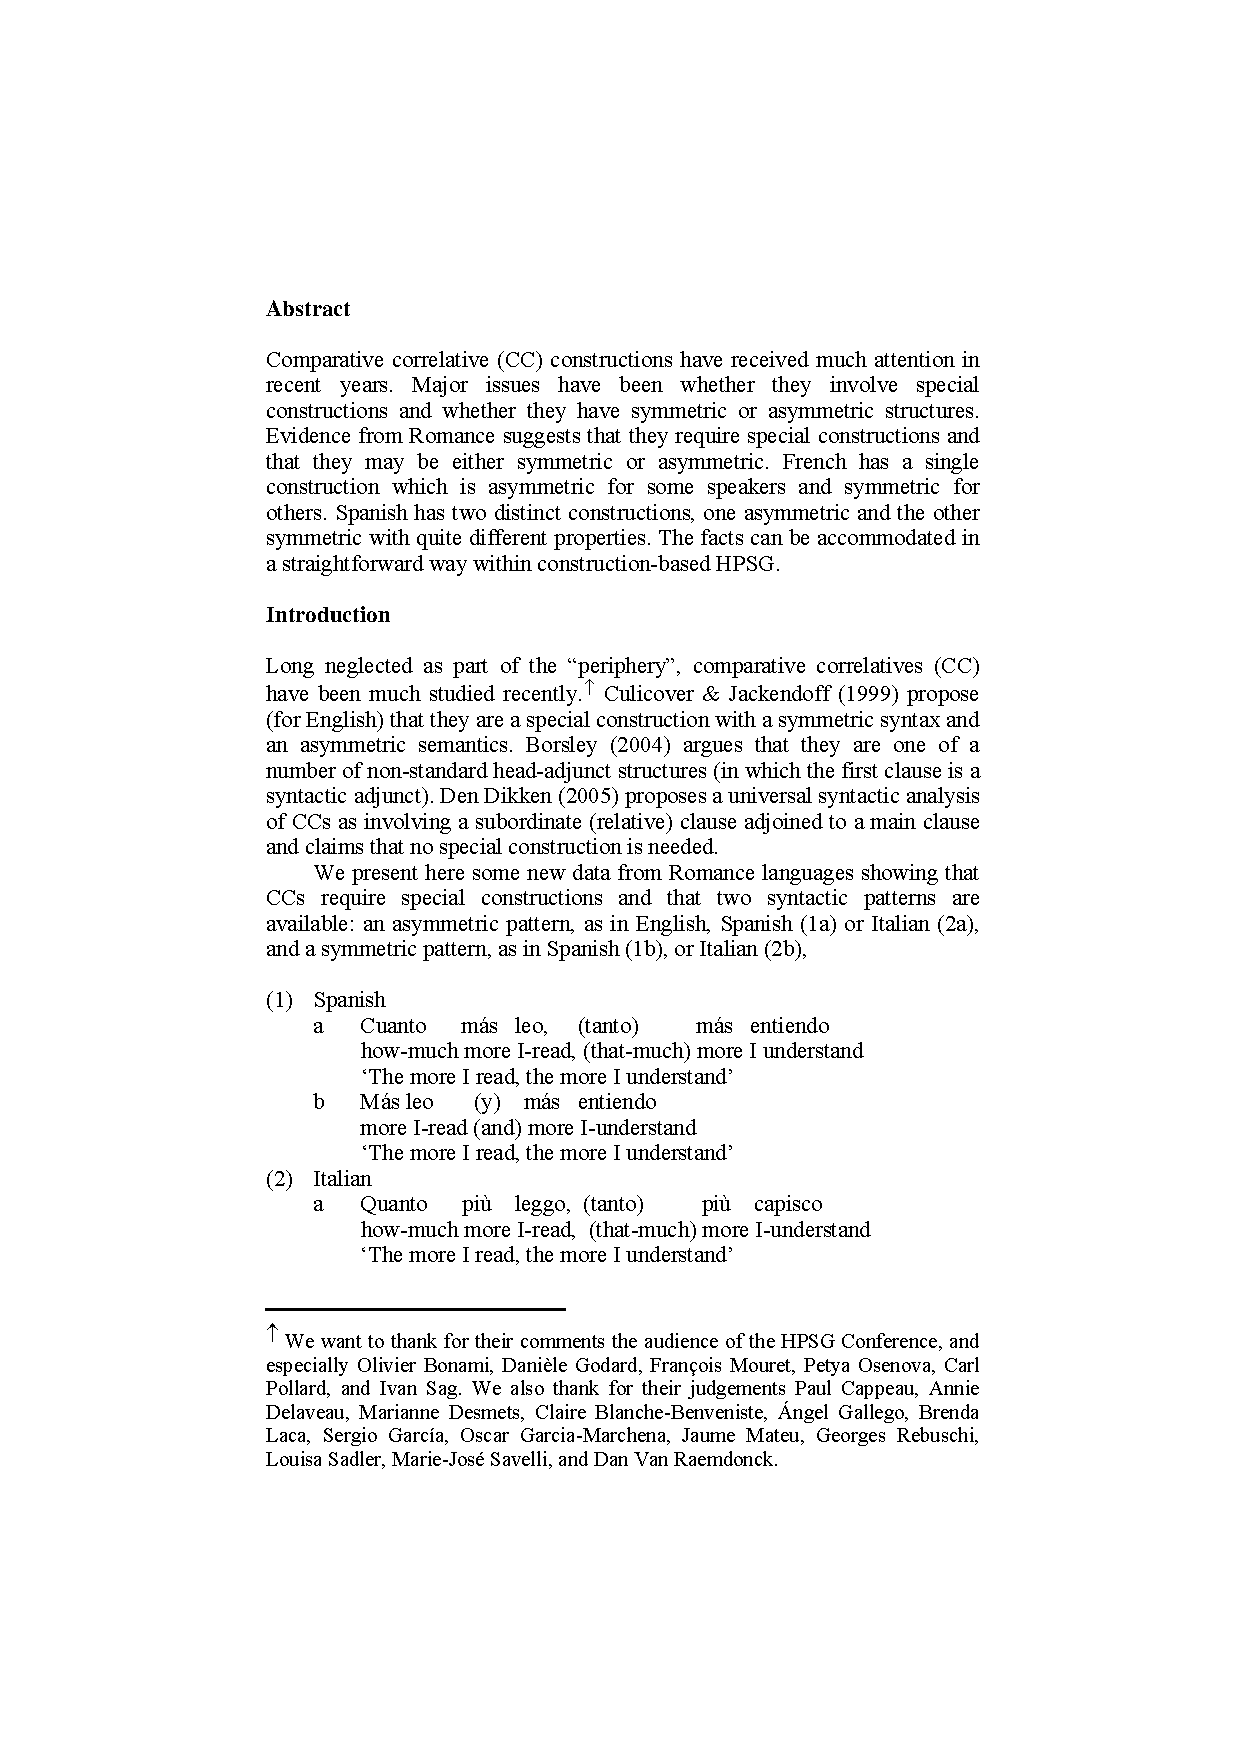
\includepdf[pages=-,pagecommand=\thispagestyle{plain}]{Includes/abe.pdf}
        \setcounter{page}{27}
        \phantomsection
        \addcontentsline{toc}{section}{Tania Avgustinova: A Functional Typology of Copular ``be'': Towards an HPSG Formalisation}
\thispagestyle{empty}

\begin{center}
  {\huge\bfseries A Functional Typology of Copular ``be'': Towards an HPSG Formalisation\par}

  \bigskip

~\\
\begingroup
\setlength{\leftskip}{0pt plus 1fill}
\setlength{\rightskip}{0pt plus 1fill}
\setlength{\parindent}{0pt}
\setlength{\parfillskip}{0pt}
  \formatauthor{Tania Avgustinova}{\begin{tabular}{@{}c@{}}DFKI\end{tabular}}

\par\endgroup

  \vspace*{8ex}

  Proceedings of the 13th International Conference on\par Head-Driven Phrase Structure Grammar

  \bigskip

  Linguistic Modelling Laboratory,\\Institute for Parallel Processing,\\Bulgarian Academy of Sciences,\\Sofia,\\Held in Varna

  \medskip

  Stefan Müller (Editor)

  \medskip

  2006

  \medskip

  CSLI Publications

  \medskip

  pages 27--38

  \medskip

  \url{http://csli-publications.stanford.edu/HPSG/2006}
\end{center}
\vfill

\noindent



\vfill
\noindent
% APA Style
Avgustinova, Tania. 2006. A Functional Typology of Copular ``be'': Towards an HPSG Formalisation. In Müller, Stefan (Ed.), \emph{{Proceedings of the 13th International Conference on Head-Driven Phrase Structure Grammar, Varna}}, 27--38. Stanford,
CA: CSLI Publications. \hfill\href{http://creativecommons.org/licenses/by/4.0/}{\includegraphics[height=.75em]{Includes/ccby.eps}}

\newpage
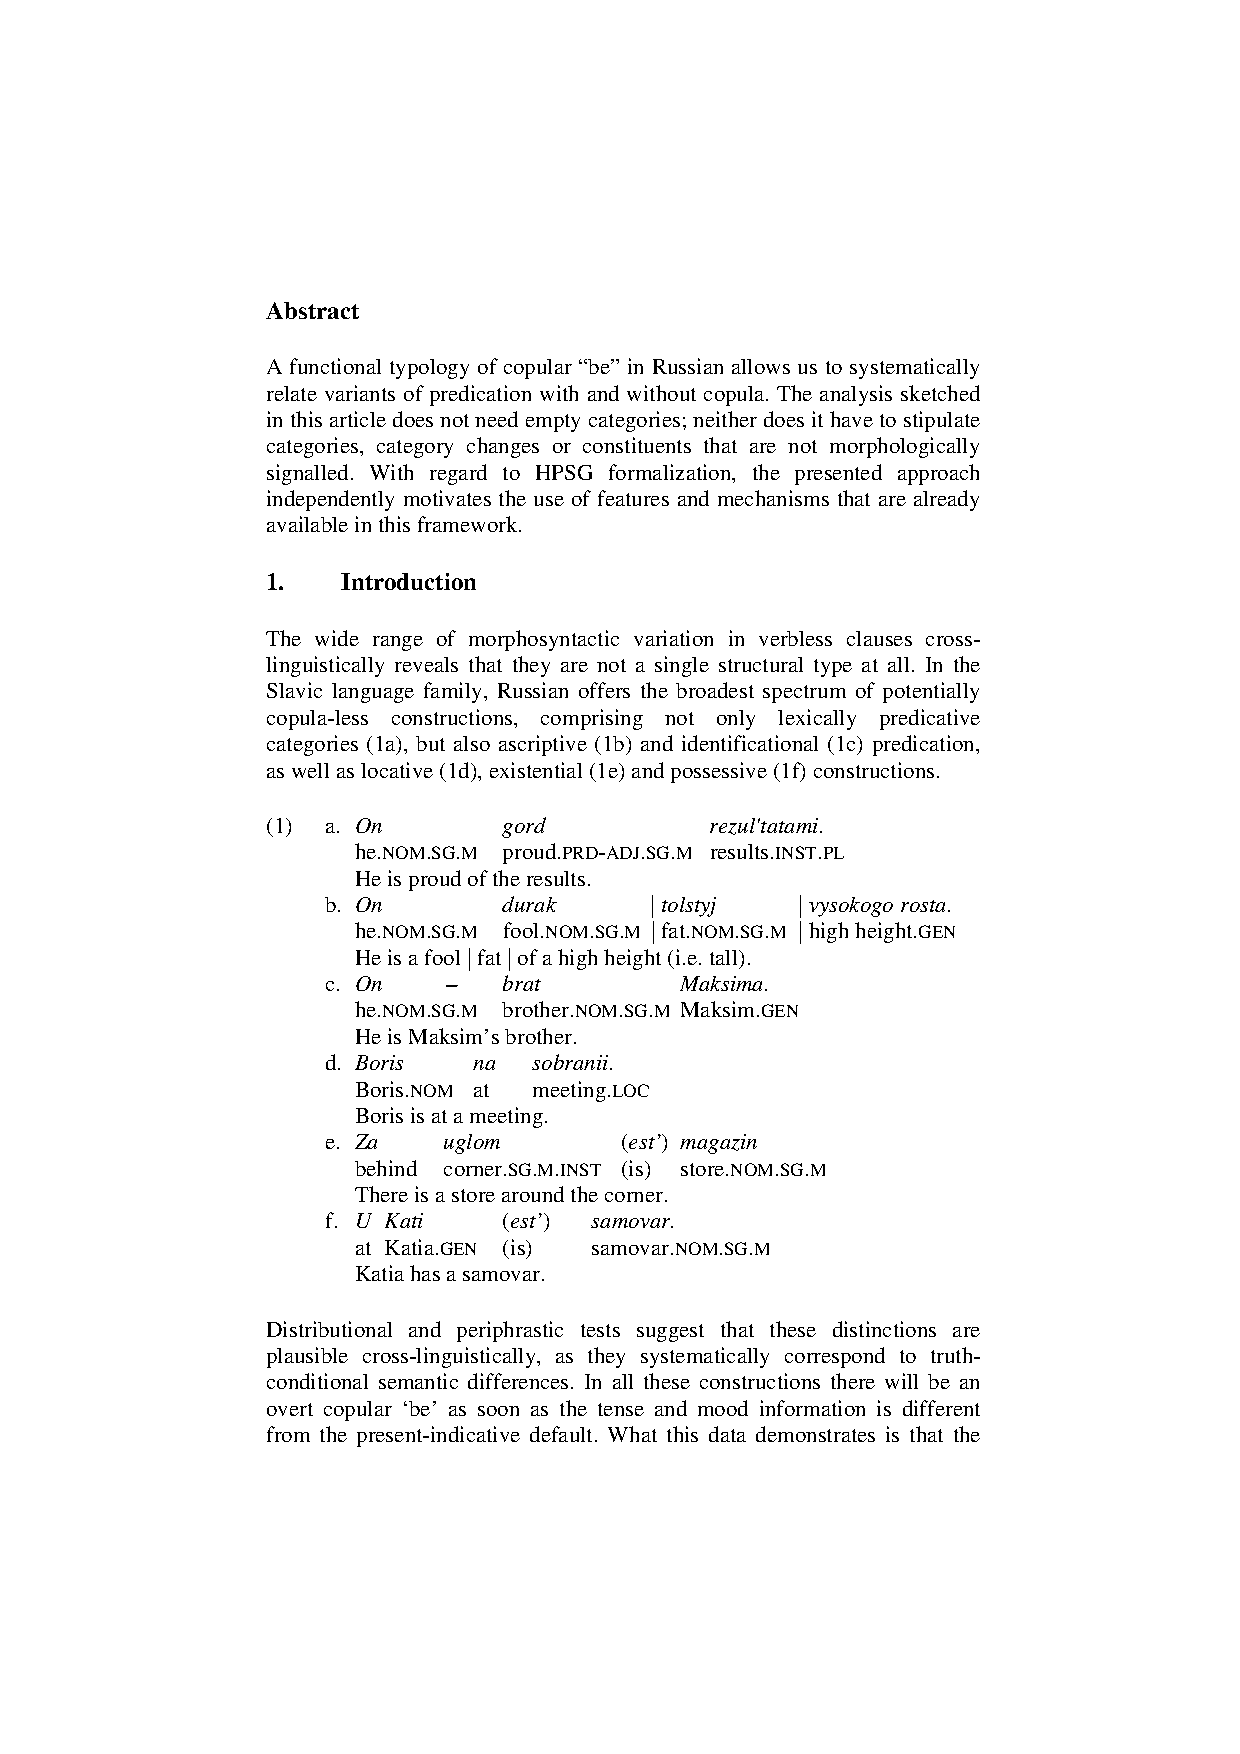
\includepdf[pages=-,pagecommand=\thispagestyle{plain}]{Includes/avgustinova.pdf}
        \setcounter{page}{39}
        \phantomsection
        \addcontentsline{toc}{section}{Olivier Bonami, Elisabeth Delais-Roussarie: Metrical Phonology in HPSG}
\thispagestyle{empty}

\begin{center}
  {\huge\bfseries Metrical Phonology in HPSG\par}

  \bigskip

~\\
\begingroup
\setlength{\leftskip}{0pt plus 1fill}
\setlength{\rightskip}{0pt plus 1fill}
\setlength{\parindent}{0pt}
\setlength{\parfillskip}{0pt}
  \formatauthor{Olivier Bonami}{\begin{tabular}{@{}c@{}}Université Paris-Sorbonne\end{tabular}}
\formatauthor{Elisabeth Delais-Roussarie}{\begin{tabular}{@{}c@{}}LLF\end{tabular}}

\par\endgroup

  \vspace*{8ex}

  Proceedings of the 13th International Conference on\par Head-Driven Phrase Structure Grammar

  \bigskip

  Linguistic Modelling Laboratory,\\Institute for Parallel Processing,\\Bulgarian Academy of Sciences,\\Sofia,\\Held in Varna

  \medskip

  Stefan Müller (Editor)

  \medskip

  2006

  \medskip

  CSLI Publications

  \medskip

  pages 39--59

  \medskip

  \url{http://csli-publications.stanford.edu/HPSG/2006}
\end{center}
\vfill

\noindent



\vfill
\noindent
% APA Style
Bonami, Olivier, \& Delais-Roussarie,  Elisabeth. 2006. Metrical Phonology in HPSG. In Müller, Stefan (Ed.), \emph{{Proceedings of the 13th International Conference on Head-Driven Phrase Structure Grammar, Varna}}, 39--59. Stanford,
CA: CSLI Publications. \hfill\href{http://creativecommons.org/licenses/by/4.0/}{\includegraphics[height=.75em]{Includes/ccby.eps}}

\newpage
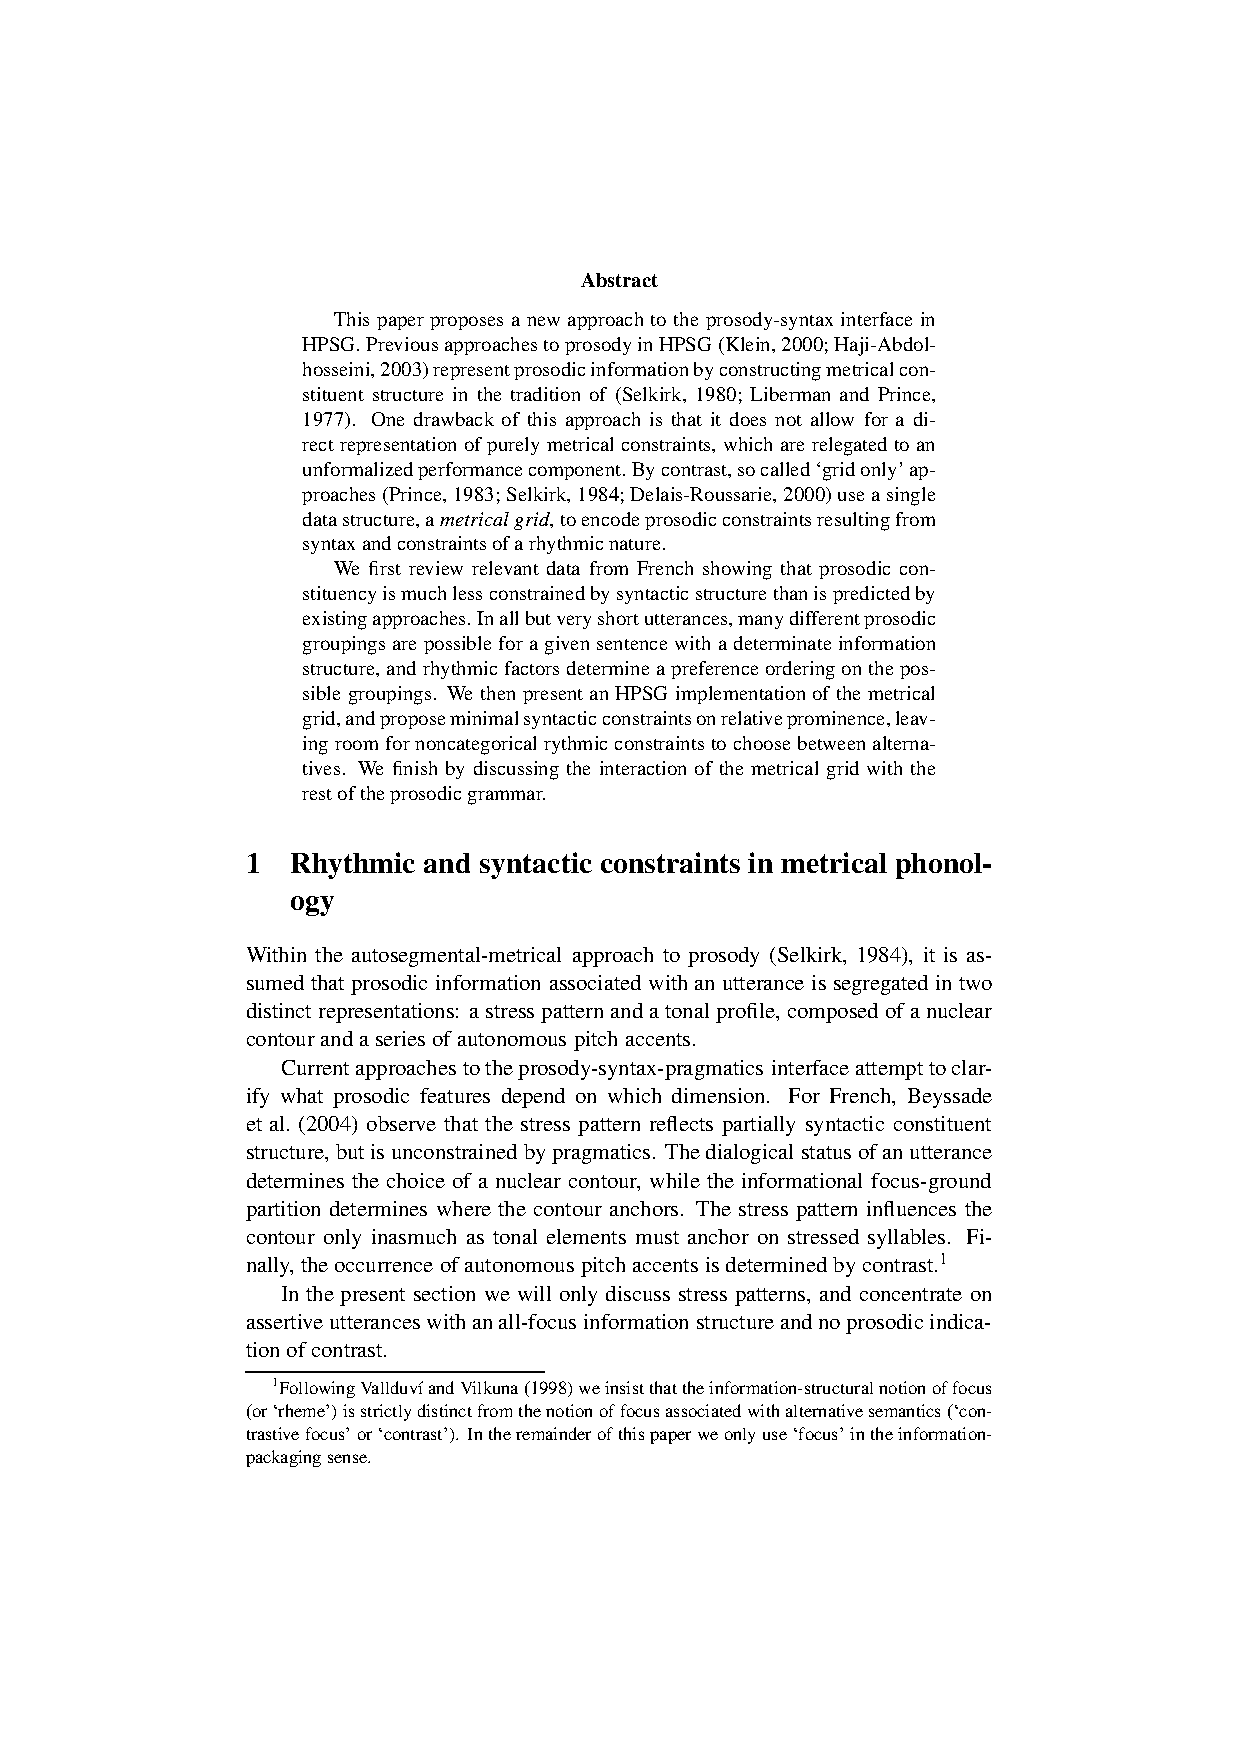
\includepdf[pages=-,pagecommand=\thispagestyle{plain}]{Includes/bonami-delais-roussarie.pdf}
        \setcounter{page}{60}
        \phantomsection
        \addcontentsline{toc}{section}{Robert D. Borsley: A Linear Approach to Negative Prominence}
\thispagestyle{empty}

\begin{center}
  {\huge\bfseries A Linear Approach to Negative Prominence\par}

  \bigskip

~\\
\begingroup
\setlength{\leftskip}{0pt plus 1fill}
\setlength{\rightskip}{0pt plus 1fill}
\setlength{\parindent}{0pt}
\setlength{\parfillskip}{0pt}
  \formatauthor{Robert D. Borsley}{\begin{tabular}{@{}c@{}}University of Essex\end{tabular}}

\par\endgroup

  \vspace*{8ex}

  Proceedings of the 13th International Conference on\par Head-Driven Phrase Structure Grammar

  \bigskip

  Linguistic Modelling Laboratory,\\Institute for Parallel Processing,\\Bulgarian Academy of Sciences,\\Sofia,\\Held in Varna

  \medskip

  Stefan Müller (Editor)

  \medskip

  2006

  \medskip

  CSLI Publications

  \medskip

  pages 60--80

  \medskip

  \url{http://csli-publications.stanford.edu/HPSG/2006}
\end{center}
\vfill

\noindent



\vfill
\noindent
% APA Style
Borsley, Robert D. 2006. A Linear Approach to Negative Prominence. In Müller, Stefan (Ed.), \emph{{Proceedings of the 13th International Conference on Head-Driven Phrase Structure Grammar, Varna}}, 60--80. Stanford,
CA: CSLI Publications. \hfill\href{http://creativecommons.org/licenses/by/4.0/}{\includegraphics[height=.75em]{Includes/ccby.eps}}

\newpage
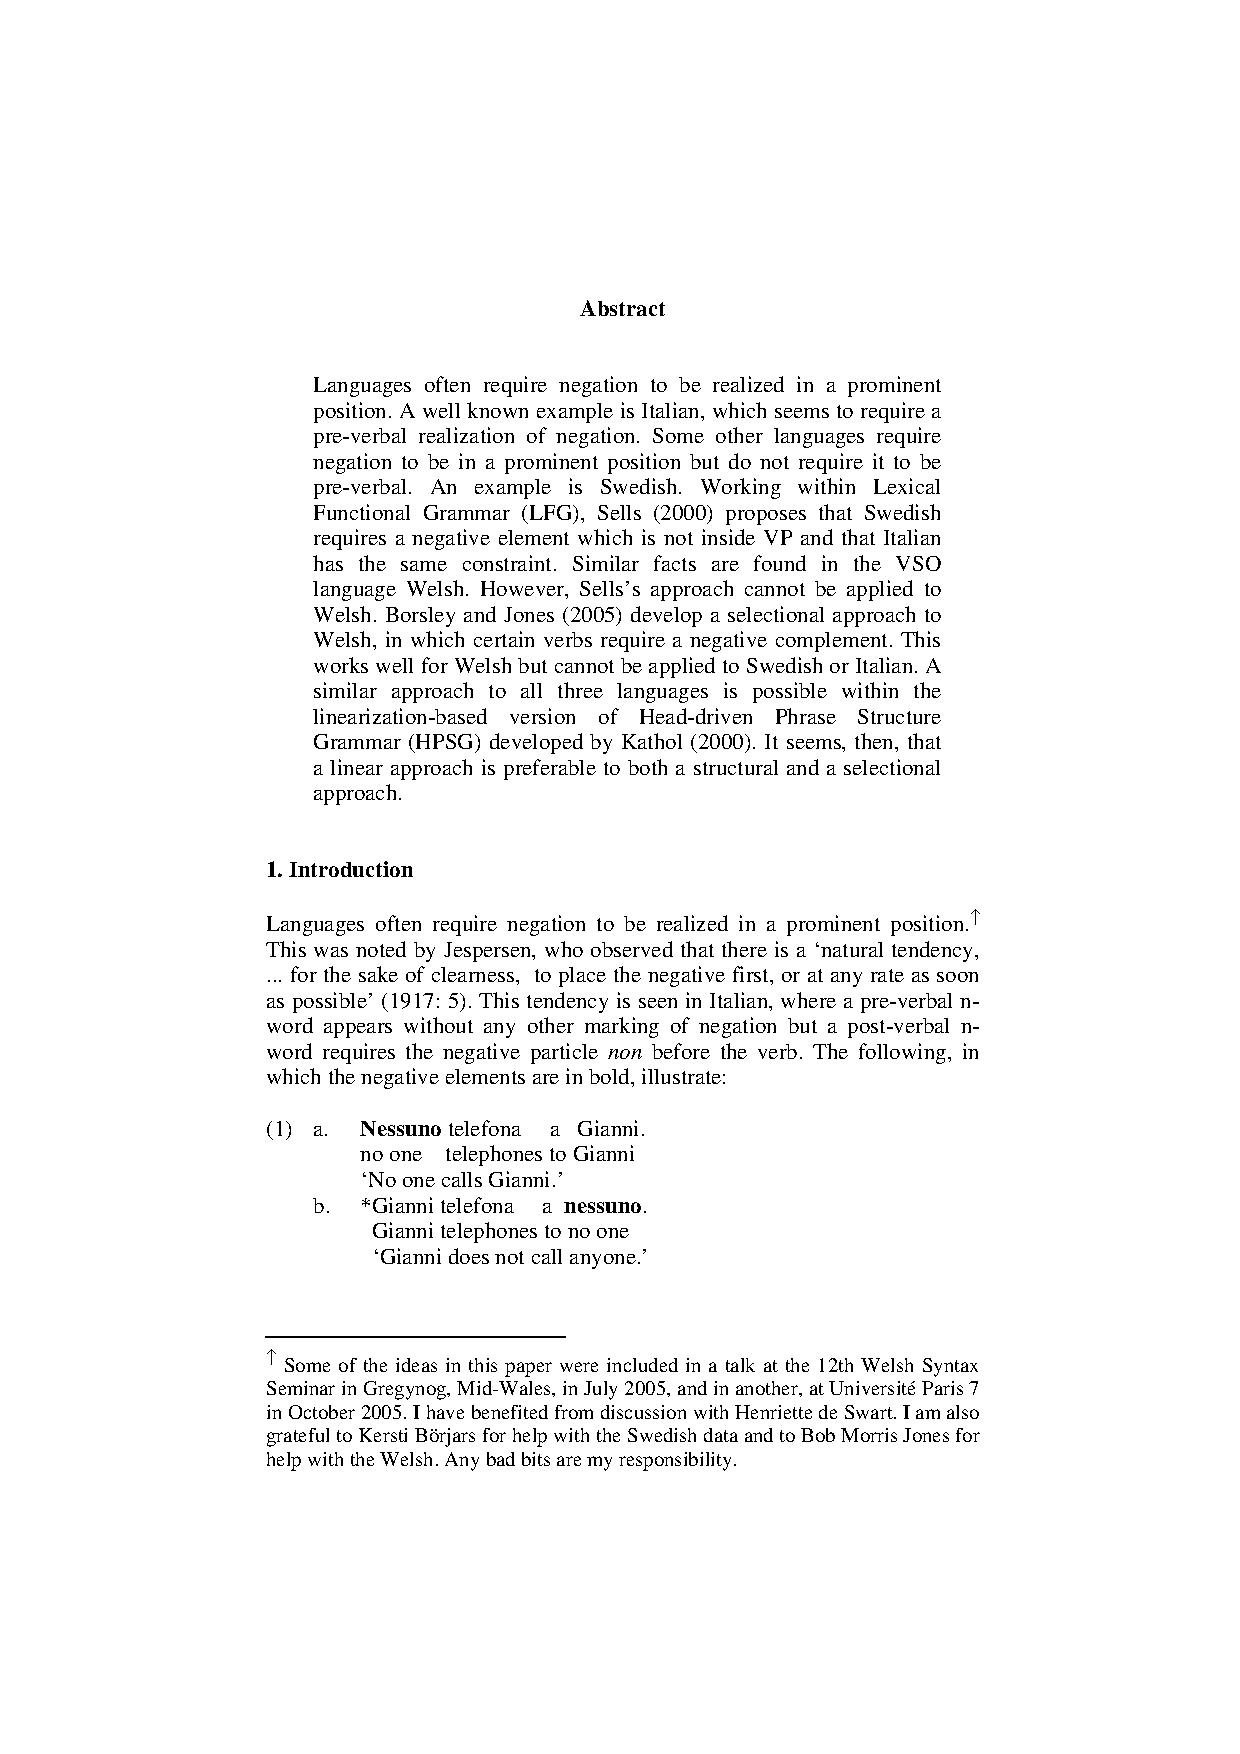
\includepdf[pages=-,pagecommand=\thispagestyle{plain}]{Includes/borsley.pdf}
        \setcounter{page}{81}
        \phantomsection
        \addcontentsline{toc}{section}{Ant{\'o}nio Branco, Francisco Costa: Noun Ellipsis without Empty Categories}
\thispagestyle{empty}

\begin{center}
  {\huge\bfseries Noun Ellipsis without Empty Categories\par}

  \bigskip

~\\
\begingroup
\setlength{\leftskip}{0pt plus 1fill}
\setlength{\rightskip}{0pt plus 1fill}
\setlength{\parindent}{0pt}
\setlength{\parfillskip}{0pt}
  \formatauthor{António Branco}{\begin{tabular}{@{}c@{}}University of Lisbon\end{tabular}}
\formatauthor{Francisco Costa}{\begin{tabular}{@{}c@{}}University of Lisbon\end{tabular}}

\par\endgroup

  \vspace*{8ex}

  Proceedings of the 13th International Conference on\par Head-Driven Phrase Structure Grammar

  \bigskip

  Linguistic Modelling Laboratory,\\Institute for Parallel Processing,\\Bulgarian Academy of Sciences,\\Sofia,\\Held in Varna

  \medskip

  Stefan Müller (Editor)

  \medskip

  2006

  \medskip

  CSLI Publications

  \medskip

  pages 81--101

  \medskip

  \url{http://csli-publications.stanford.edu/HPSG/2006}
\end{center}
\vfill

\noindent



\vfill
\noindent
% APA Style
Branco, António, \& Costa, Francisco. 2006. Noun Ellipsis without Empty Categories. In Müller, Stefan (Ed.), \emph{{Proceedings of the 13th International Conference on Head-Driven Phrase Structure Grammar, Varna}}, 81--101. Stanford,
CA: CSLI Publications. \hfill\href{http://creativecommons.org/licenses/by/4.0/}{\includegraphics[height=.75em]{Includes/ccby.eps}}

\newpage
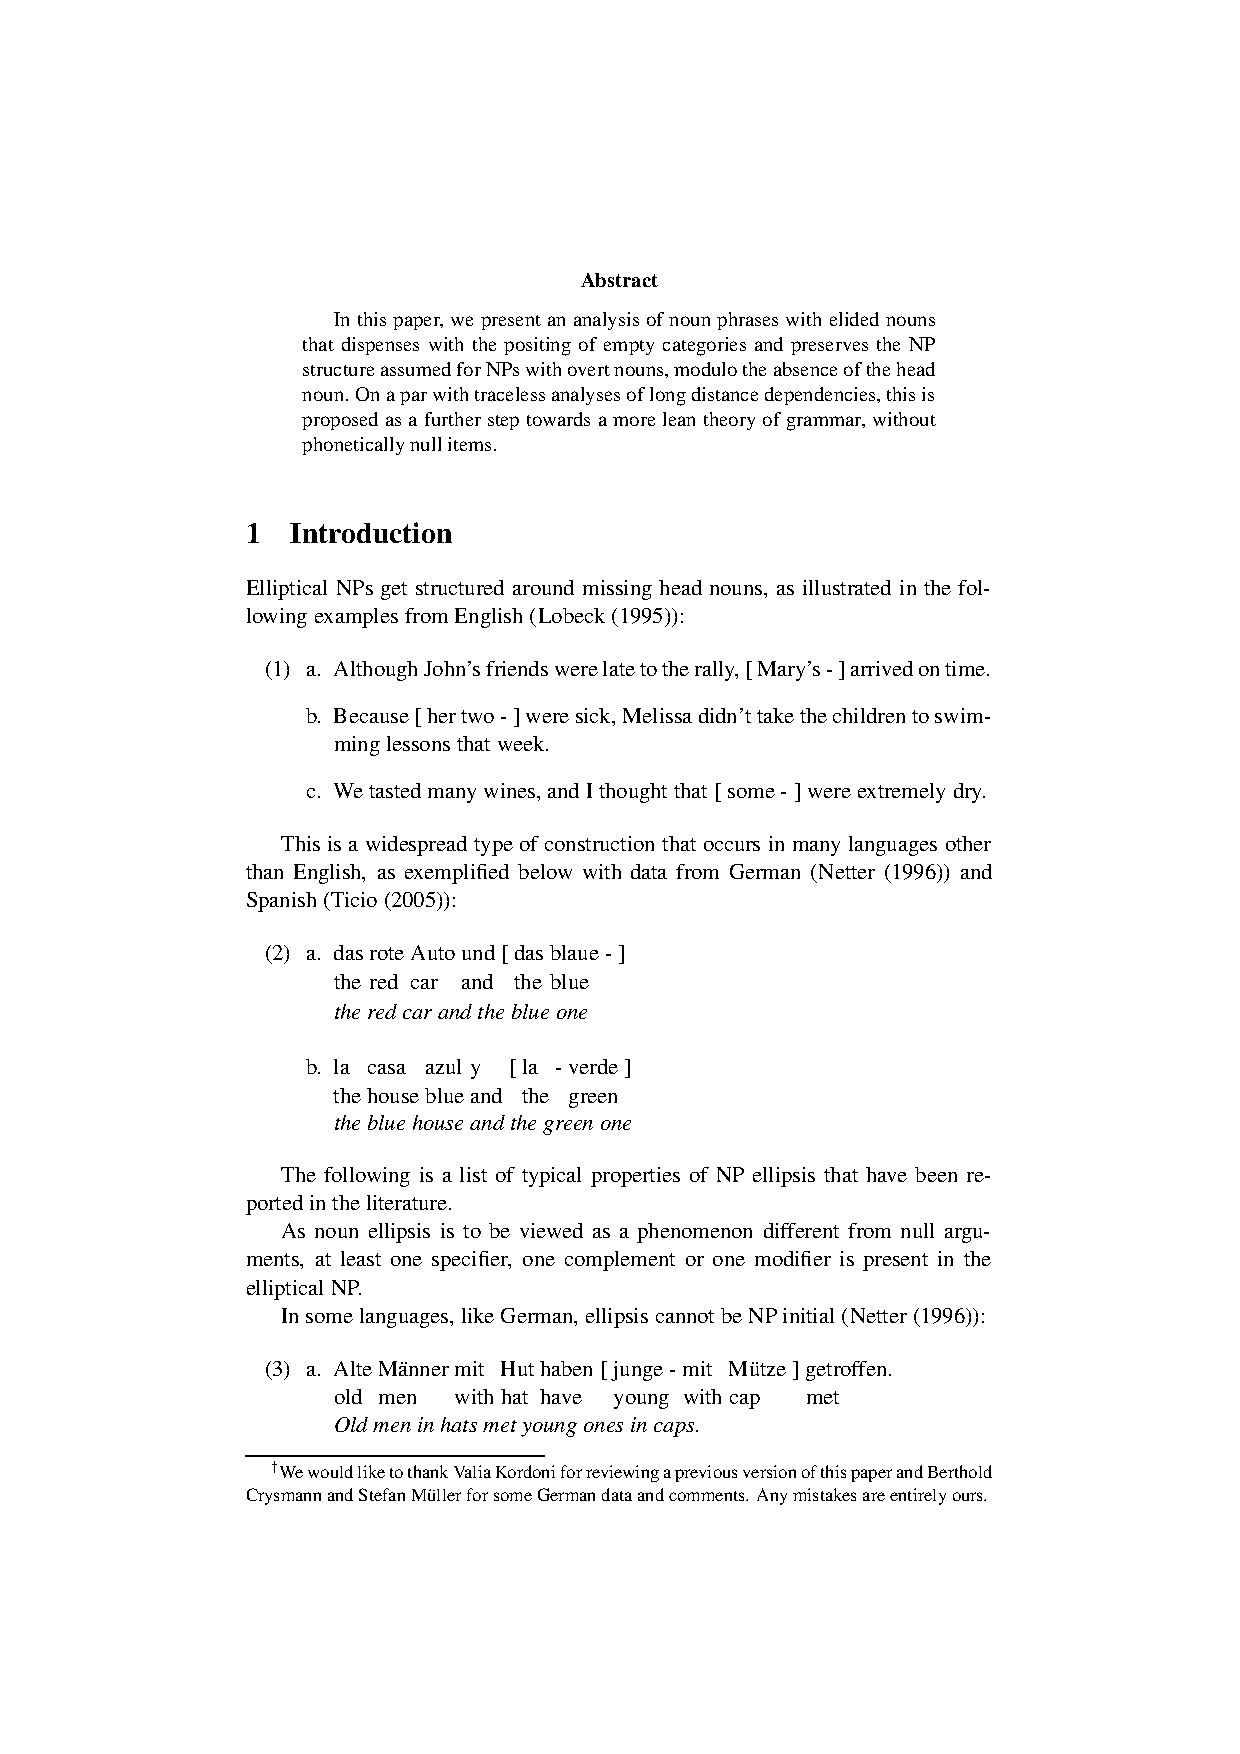
\includepdf[pages=-,pagecommand=\thispagestyle{plain}]{Includes/branco-costa.pdf}
        \setcounter{page}{102}
        \phantomsection
        \addcontentsline{toc}{section}{Rui P. Chaves: Coordination of Unlikes without Unlike Categories}
\thispagestyle{empty}

\begin{center}
  {\huge\bfseries Coordination of Unlikes without Unlike Categories\par}

  \bigskip

~\\
\begingroup
\setlength{\leftskip}{0pt plus 1fill}
\setlength{\rightskip}{0pt plus 1fill}
\setlength{\parindent}{0pt}
\setlength{\parfillskip}{0pt}
  \formatauthor{Rui P. Chaves}{\begin{tabular}{@{}c@{}}Centro de Linguística da Universidade de Lisboa\end{tabular}}

\par\endgroup

  \vspace*{8ex}

  Proceedings of the 13th International Conference on\par Head-Driven Phrase Structure Grammar

  \bigskip

  Linguistic Modelling Laboratory,\\Institute for Parallel Processing,\\Bulgarian Academy of Sciences,\\Sofia,\\Held in Varna

  \medskip

  Stefan Müller (Editor)

  \medskip

  2006

  \medskip

  CSLI Publications

  \medskip

  pages 102--122

  \medskip

  \url{http://csli-publications.stanford.edu/HPSG/2006}
\end{center}
\vfill

\noindent



\vfill
\noindent
% APA Style
Chaves, Rui P. 2006. Coordination of Unlikes without Unlike Categories. In Müller, Stefan (Ed.), \emph{{Proceedings of the 13th International Conference on Head-Driven Phrase Structure Grammar, Varna}}, 102--122. Stanford,
CA: CSLI Publications. \hfill\href{http://creativecommons.org/licenses/by/4.0/}{\includegraphics[height=.75em]{Includes/ccby.eps}}

\newpage
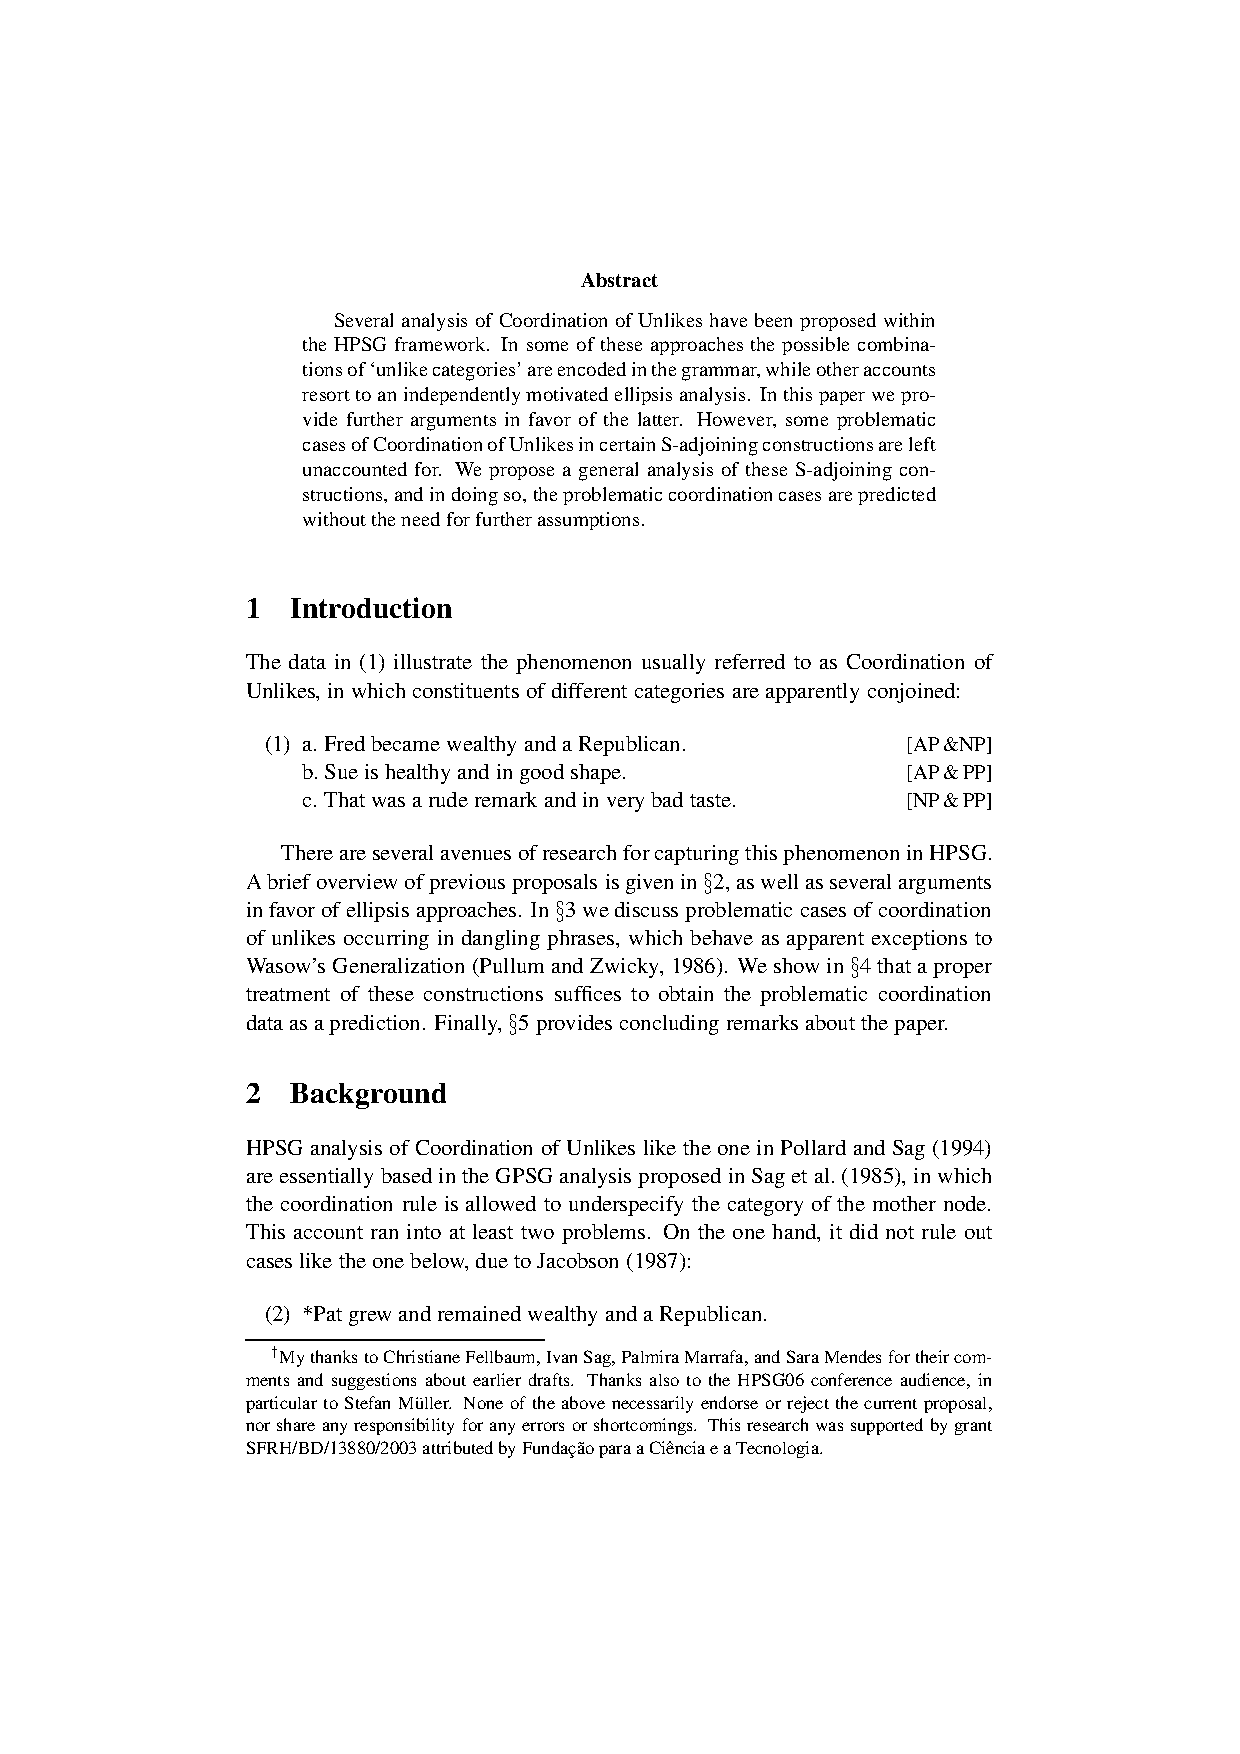
\includepdf[pages=-,pagecommand=\thispagestyle{plain}]{Includes/chaves.pdf}
        \setcounter{page}{123}
        \phantomsection
        \addcontentsline{toc}{section}{Berthold Crysmann: Floating Affixes in Polish}
\thispagestyle{empty}

\begin{center}
  {\huge\bfseries Floating Affixes in Polish\par}

  \bigskip

~\\
\begingroup
\setlength{\leftskip}{0pt plus 1fill}
\setlength{\rightskip}{0pt plus 1fill}
\setlength{\parindent}{0pt}
\setlength{\parfillskip}{0pt}
  \formatauthor{Berthold Crysmann}{\begin{tabular}{@{}c@{}}German Research Centre for Artificial Intelligence (DFKI)\end{tabular}}

\par\endgroup

  \vspace*{8ex}

  Proceedings of the 13th International Conference on\par Head-Driven Phrase Structure Grammar

  \bigskip

  Linguistic Modelling Laboratory,\\Institute for Parallel Processing,\\Bulgarian Academy of Sciences,\\Sofia,\\Held in Varna

  \medskip

  Stefan Müller (Editor)

  \medskip

  2006

  \medskip

  CSLI Publications

  \medskip

  pages 123--139

  \medskip

  \url{http://csli-publications.stanford.edu/HPSG/2006}
\end{center}
\vfill

\noindent



\vfill
\noindent
% APA Style
Crysmann, Berthold. 2006. Floating Affixes in Polish. In Müller, Stefan (Ed.), \emph{{Proceedings of the 13th International Conference on Head-Driven Phrase Structure Grammar, Varna}}, 123--139. Stanford,
CA: CSLI Publications. \hfill\href{http://creativecommons.org/licenses/by/4.0/}{\includegraphics[height=.75em]{Includes/ccby.eps}}

\newpage
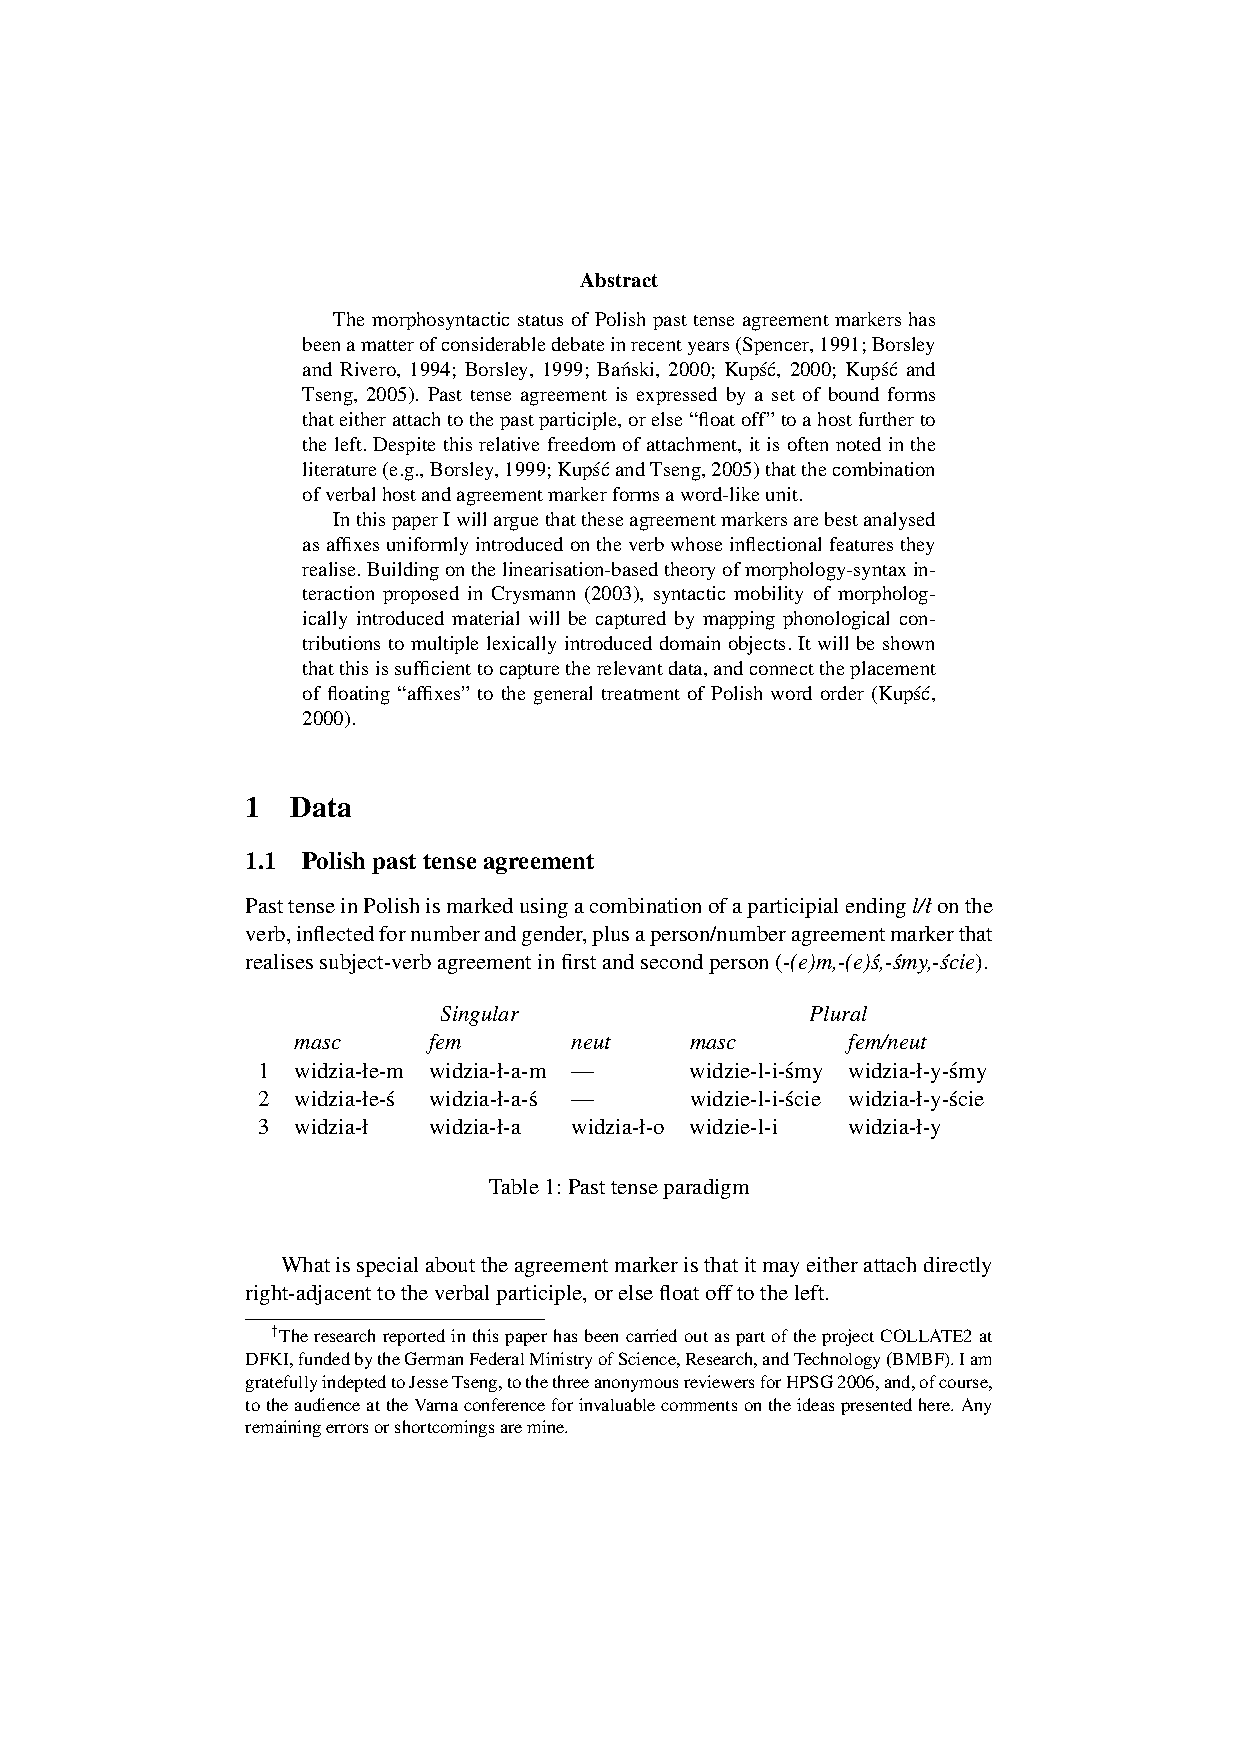
\includepdf[pages=-,pagecommand=\thispagestyle{plain}]{Includes/crysmann.pdf}
        \setcounter{page}{140}
        \phantomsection
        \addcontentsline{toc}{section}{Maria Flouraki: Constraining Aspectual Composition}
\thispagestyle{empty}

\begin{center}
  {\huge\bfseries Constraining Aspectual Composition\par}

  \bigskip

~\\
\begingroup
\setlength{\leftskip}{0pt plus 1fill}
\setlength{\rightskip}{0pt plus 1fill}
\setlength{\parindent}{0pt}
\setlength{\parfillskip}{0pt}
  \formatauthor{Maria Flouraki}{\begin{tabular}{@{}c@{}}University of Essex\end{tabular}}

\par\endgroup

  \vspace*{8ex}

  Proceedings of the 13th International Conference on\par Head-Driven Phrase Structure Grammar

  \bigskip

  Linguistic Modelling Laboratory,\\Institute for Parallel Processing,\\Bulgarian Academy of Sciences,\\Sofia,\\Held in Varna

  \medskip

  Stefan Müller (Editor)

  \medskip

  2006

  \medskip

  CSLI Publications

  \medskip

  pages 140--157

  \medskip

  \url{http://csli-publications.stanford.edu/HPSG/2006}
\end{center}
\vfill

\noindent



\vfill
\noindent
% APA Style
Flouraki, Maria. 2006. Constraining Aspectual Composition. In Müller, Stefan (Ed.), \emph{{Proceedings of the 13th International Conference on Head-Driven Phrase Structure Grammar, Varna}}, 140--157. Stanford,
CA: CSLI Publications. \hfill\href{http://creativecommons.org/licenses/by/4.0/}{\includegraphics[height=.75em]{Includes/ccby.eps}}

\newpage
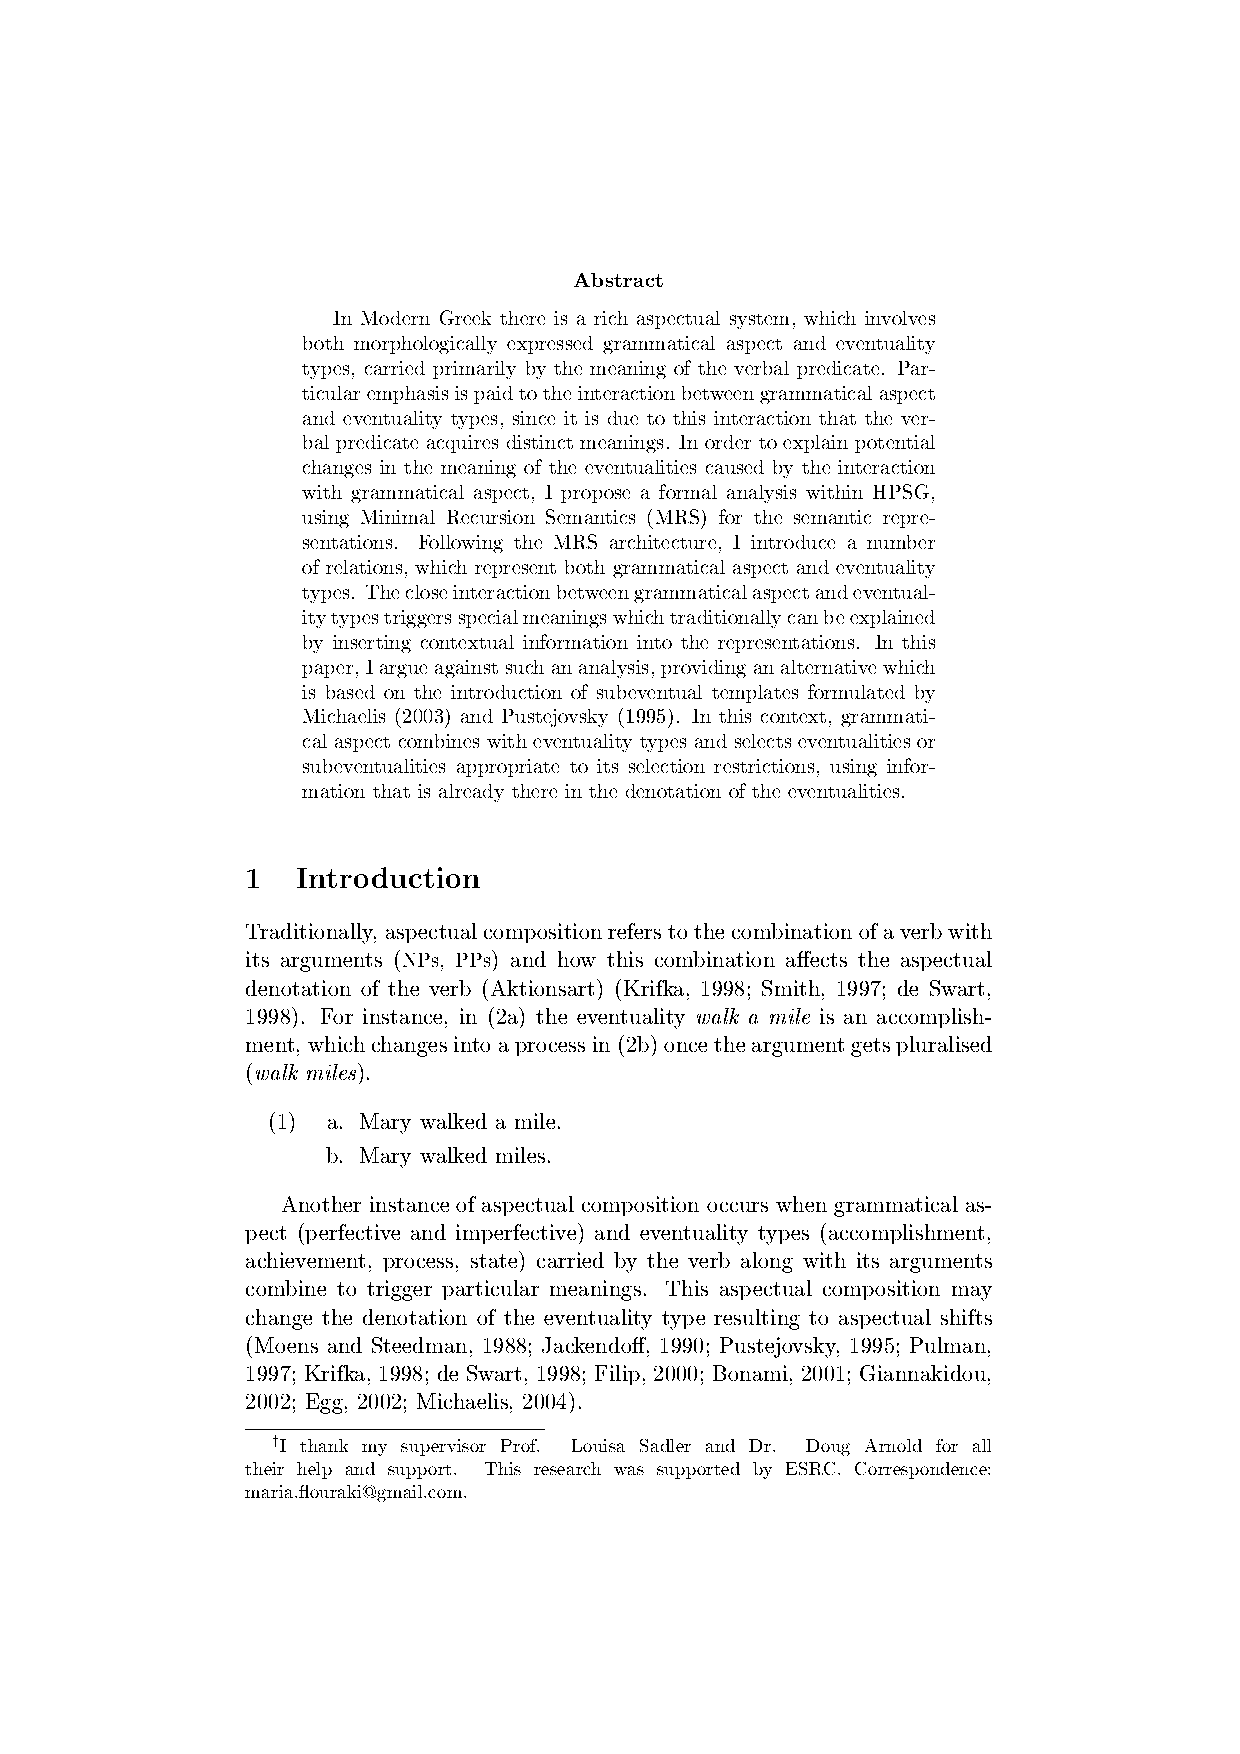
\includepdf[pages=-,pagecommand=\thispagestyle{plain}]{Includes/flouraki.pdf}
        \setcounter{page}{158}
        \phantomsection
        \addcontentsline{toc}{section}{Antske Fokkens, Valia Kordoni: Control, Raising and Case: from the perspective of passives}
\thispagestyle{empty}

\begin{center}
  {\huge\bfseries Control, Raising and Case: from the perspective of passives\par}

  \bigskip

~\\
\begingroup
\setlength{\leftskip}{0pt plus 1fill}
\setlength{\rightskip}{0pt plus 1fill}
\setlength{\parindent}{0pt}
\setlength{\parfillskip}{0pt}
  \formatauthor{Antske Fokkens}{\begin{tabular}{@{}c@{}}Dept. of Computational Linguistics,Saarland University\end{tabular}}
\formatauthor{Valia Kordoni}{\begin{tabular}{@{}c@{}}Dept. of Computational Linguistics,Saarland University\end{tabular}}

\par\endgroup

  \vspace*{8ex}

  Proceedings of the 13th International Conference on\par Head-Driven Phrase Structure Grammar

  \bigskip

  Linguistic Modelling Laboratory,\\Institute for Parallel Processing,\\Bulgarian Academy of Sciences,\\Sofia,\\Held in Varna

  \medskip

  Stefan Müller (Editor)

  \medskip

  2006

  \medskip

  CSLI Publications

  \medskip

  pages 158--173

  \medskip

  \url{http://csli-publications.stanford.edu/HPSG/2006}
\end{center}
\vfill

\noindent



\vfill
\noindent
% APA Style
Fokkens, Antske, \& Kordoni,  Valia. 2006. Control, Raising and Case: from the perspective of passives. In Müller, Stefan (Ed.), \emph{{Proceedings of the 13th International Conference on Head-Driven Phrase Structure Grammar, Varna}}, 158--173. Stanford,
CA: CSLI Publications. \hfill\href{http://creativecommons.org/licenses/by/4.0/}{\includegraphics[height=.75em]{Includes/ccby.eps}}

\newpage
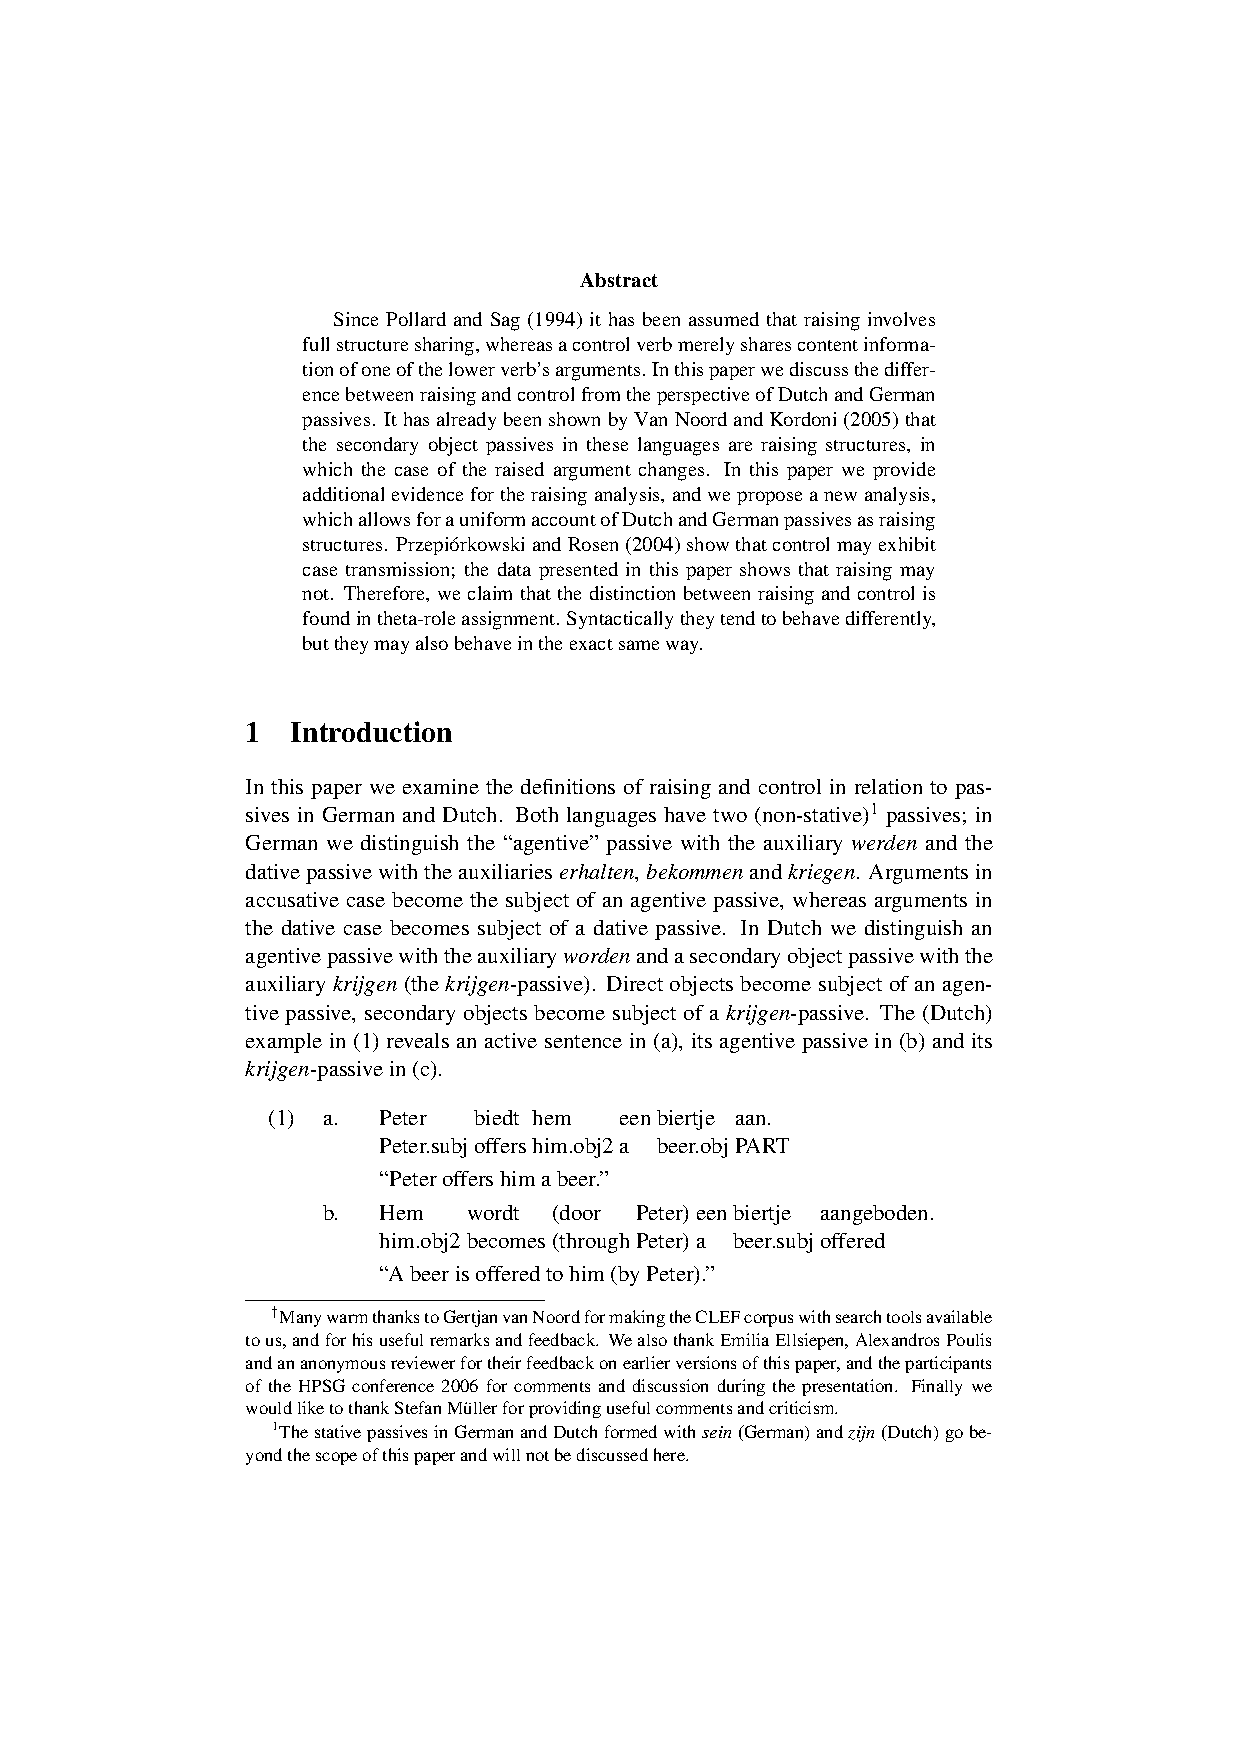
\includepdf[pages=-,pagecommand=\thispagestyle{plain}]{Includes/fokkens-kordoni.pdf}
        \setcounter{page}{174}
        \phantomsection
        \addcontentsline{toc}{section}{Dani\`{e}le Godard, Jean-Marie Marandin: Reinforcing Negation: the case of Italian}
\thispagestyle{empty}

\begin{center}
  {\huge\bfseries Reinforcing Negation: the case of Italian\par}

  \bigskip

~\\
\begingroup
\setlength{\leftskip}{0pt plus 1fill}
\setlength{\rightskip}{0pt plus 1fill}
\setlength{\parindent}{0pt}
\setlength{\parfillskip}{0pt}
  \formatauthor{Danièle Godard}{\begin{tabular}{@{}c@{}}CNRS, Université Paris 7\end{tabular}}
\formatauthor{Jean-Marie Marandin}{\begin{tabular}{@{}c@{}}CNRS, Université Paris 7\end{tabular}}

\par\endgroup

  \vspace*{8ex}

  Proceedings of the 13th International Conference on\par Head-Driven Phrase Structure Grammar

  \bigskip

  Linguistic Modelling Laboratory,\\Institute for Parallel Processing,\\Bulgarian Academy of Sciences,\\Sofia,\\Held in Varna

  \medskip

  Stefan Müller (Editor)

  \medskip

  2006

  \medskip

  CSLI Publications

  \medskip

  pages 174--194

  \medskip

  \url{http://csli-publications.stanford.edu/HPSG/2006}
\end{center}
\vfill

\noindent



\vfill
\noindent
% APA Style
Godard, Danièle, \& Marandin, Jean-Marie. 2006. Reinforcing Negation: the case of Italian. In Müller, Stefan (Ed.), \emph{{Proceedings of the 13th International Conference on Head-Driven Phrase Structure Grammar, Varna}}, 174--194. Stanford,
CA: CSLI Publications. \hfill\href{http://creativecommons.org/licenses/by/4.0/}{\includegraphics[height=.75em]{Includes/ccby.eps}}

\newpage
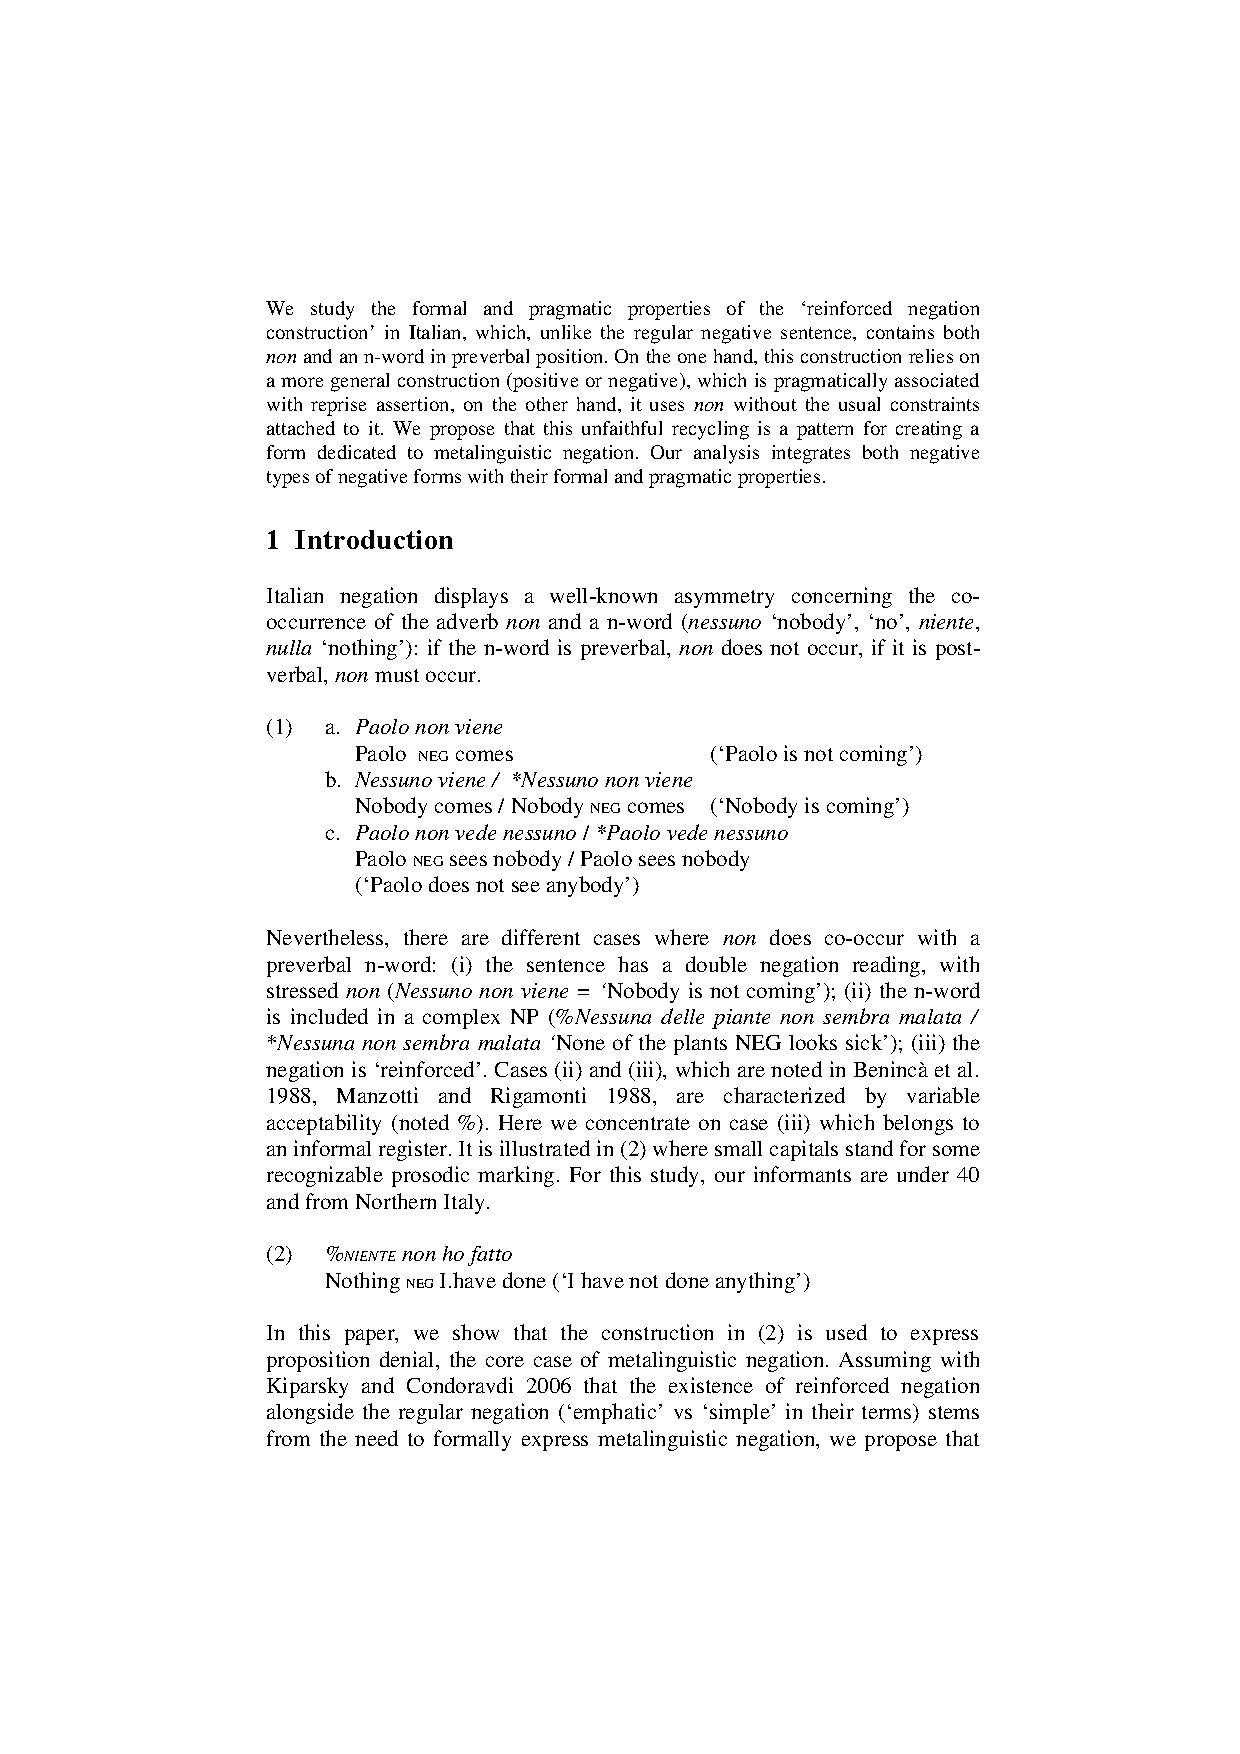
\includepdf[pages=-,pagecommand=\thispagestyle{plain}]{Includes/godard-marandin.pdf}
        \setcounter{page}{195}
        \phantomsection
        \addcontentsline{toc}{section}{Hyun-Jong Hahm: Person and Number Agreement in American Sign Language}
\thispagestyle{empty}

\begin{center}
  {\huge\bfseries Person and Number Agreement in American Sign Language\par}

  \bigskip

~\\
\begingroup
\setlength{\leftskip}{0pt plus 1fill}
\setlength{\rightskip}{0pt plus 1fill}
\setlength{\parindent}{0pt}
\setlength{\parfillskip}{0pt}
  \formatauthor{Hyun-Jong Hahm}{\begin{tabular}{@{}c@{}}The University of Texas at Austin\end{tabular}}

\par\endgroup

  \vspace*{8ex}

  Proceedings of the 13th International Conference on\par Head-Driven Phrase Structure Grammar

  \bigskip

  Linguistic Modelling Laboratory,\\Institute for Parallel Processing,\\Bulgarian Academy of Sciences,\\Sofia,\\Held in Varna

  \medskip

  Stefan Müller (Editor)

  \medskip

  2006

  \medskip

  CSLI Publications

  \medskip

  pages 195--211

  \medskip

  \url{http://csli-publications.stanford.edu/HPSG/2006}
\end{center}
\vfill

\noindent



\vfill
\noindent
% APA Style
Hahm, Hyun-Jong. 2006. Person and Number Agreement in American Sign Language. In Müller, Stefan (Ed.), \emph{{Proceedings of the 13th International Conference on Head-Driven Phrase Structure Grammar, Varna}}, 195--211. Stanford,
CA: CSLI Publications. \hfill\href{http://creativecommons.org/licenses/by/4.0/}{\includegraphics[height=.75em]{Includes/ccby.eps}}

\newpage
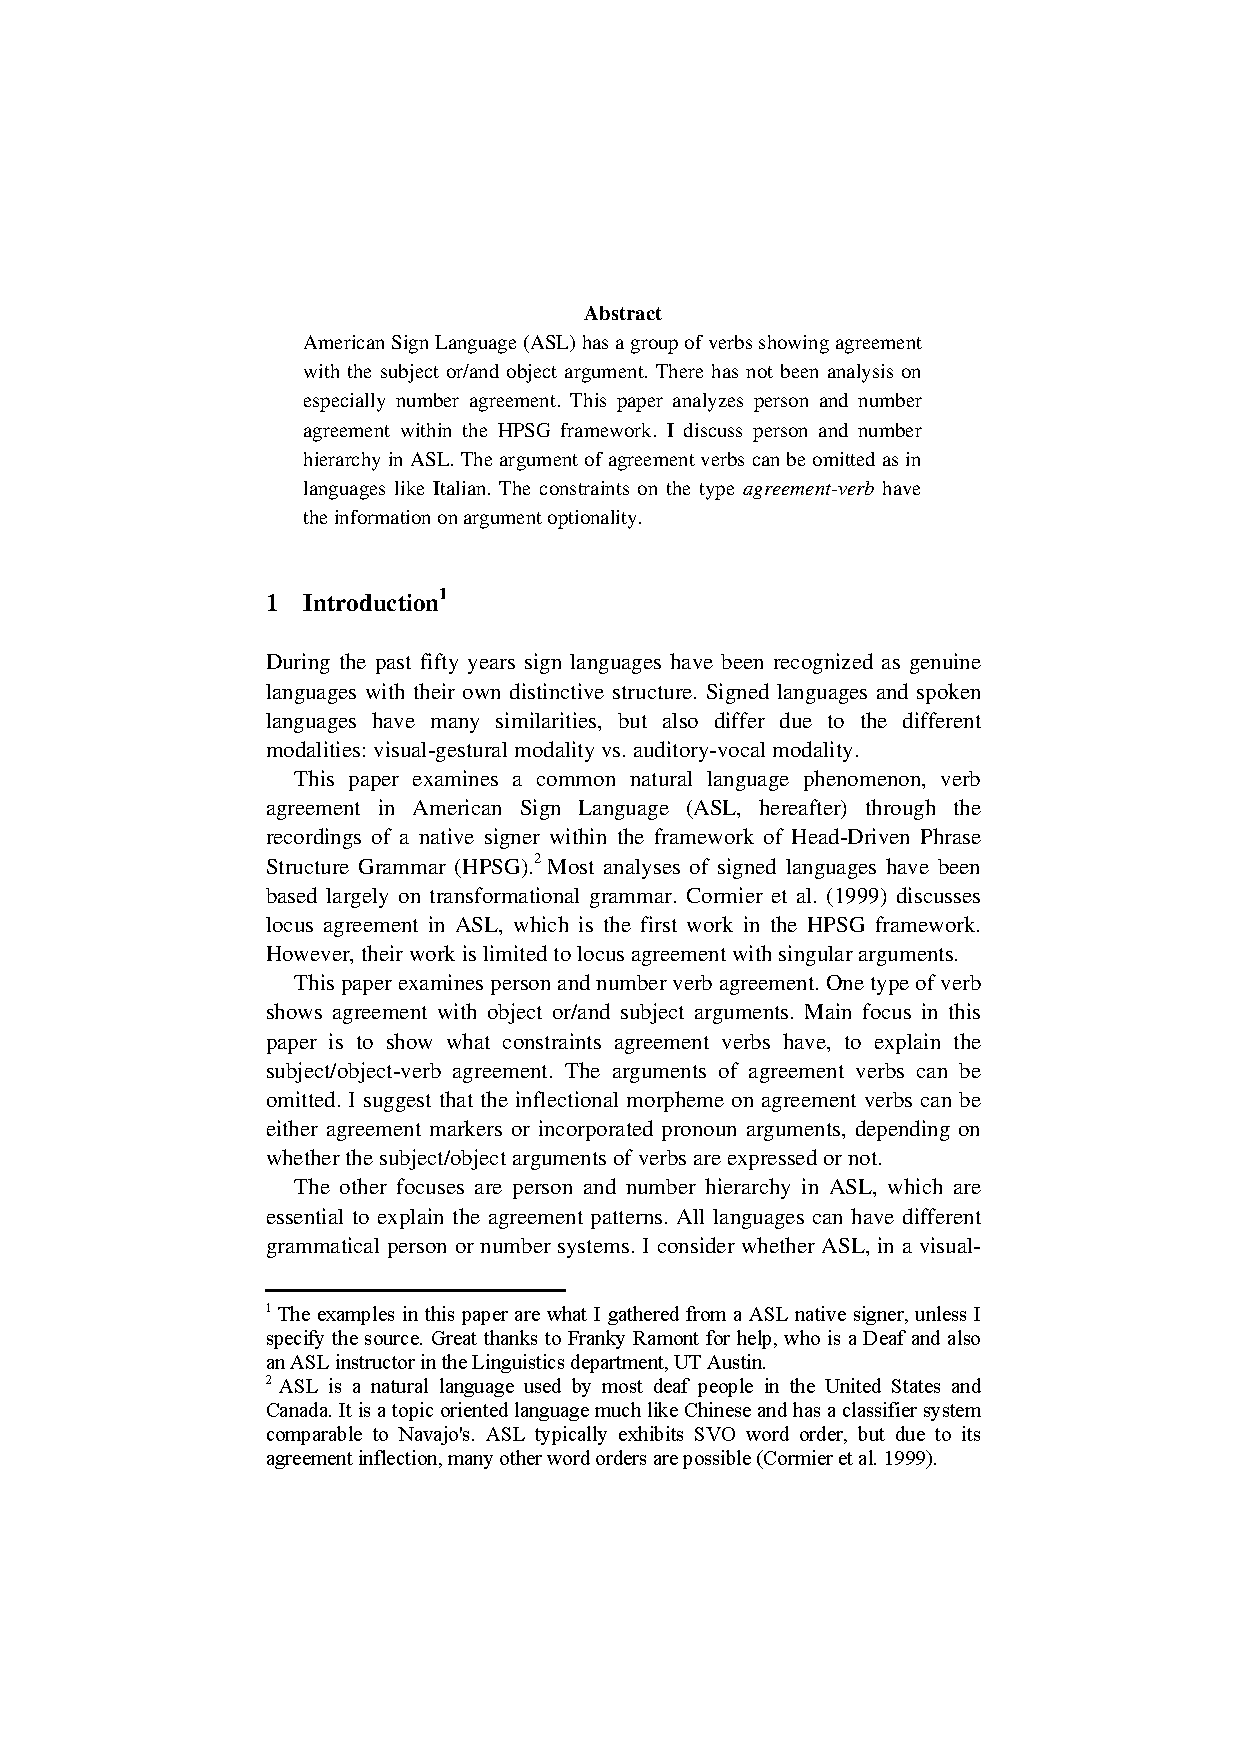
\includepdf[pages=-,pagecommand=\thispagestyle{plain}]{Includes/hahm.pdf}
        \setcounter{page}{212}
        \phantomsection
        \addcontentsline{toc}{section}{Takafumi Maekawa: Long and Short Adjunct Fronting in HPSG}
\thispagestyle{empty}

\begin{center}
  {\huge\bfseries Long and Short Adjunct Fronting in HPSG\par}

  \bigskip

~\\
\begingroup
\setlength{\leftskip}{0pt plus 1fill}
\setlength{\rightskip}{0pt plus 1fill}
\setlength{\parindent}{0pt}
\setlength{\parfillskip}{0pt}
  \formatauthor{Takafumi Maekawa}{\begin{tabular}{@{}c@{}}Department of Language and Linguistics University of Essex\end{tabular}}

\par\endgroup

  \vspace*{8ex}

  Proceedings of the 13th International Conference on\par Head-Driven Phrase Structure Grammar

  \bigskip

  Linguistic Modelling Laboratory,\\Institute for Parallel Processing,\\Bulgarian Academy of Sciences,\\Sofia,\\Held in Varna

  \medskip

  Stefan Müller (Editor)

  \medskip

  2006

  \medskip

  CSLI Publications

  \medskip

  pages 212--227

  \medskip

  \url{http://csli-publications.stanford.edu/HPSG/2006}
\end{center}
\vfill

\noindent



\vfill
\noindent
% APA Style
Maekawa, Takafumi. 2006. Long and Short Adjunct Fronting in HPSG. In Müller, Stefan (Ed.), \emph{{Proceedings of the 13th International Conference on Head-Driven Phrase Structure Grammar, Varna}}, 212--227. Stanford,
CA: CSLI Publications. \hfill\href{http://creativecommons.org/licenses/by/4.0/}{\includegraphics[height=.75em]{Includes/ccby.eps}}

\newpage
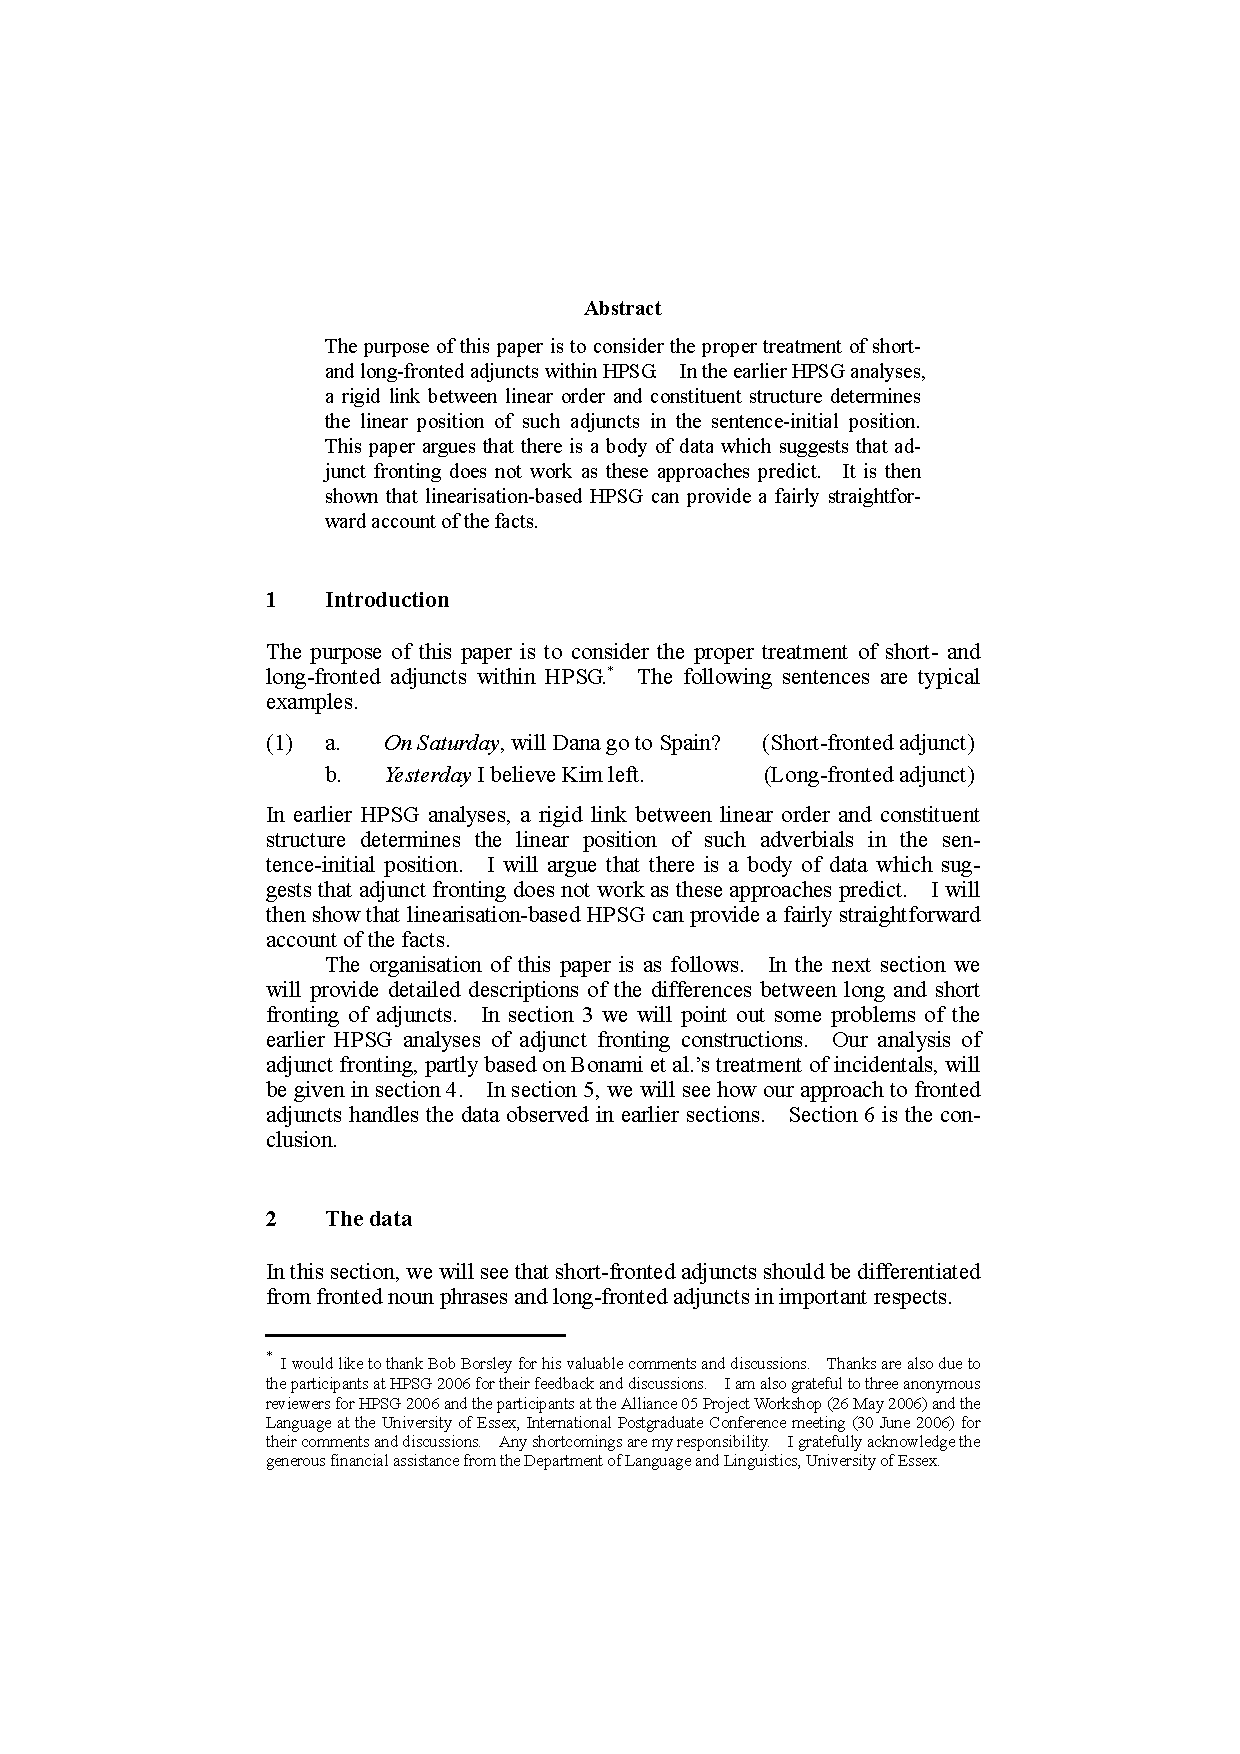
\includepdf[pages=-,pagecommand=\thispagestyle{plain}]{Includes/maekawa.pdf}
        \setcounter{page}{228}
        \phantomsection
        \addcontentsline{toc}{section}{Nurit Melnik: Hybrid Agreement as a Conflict Resolution Strategy}
\thispagestyle{empty}

\begin{center}
  {\huge\bfseries Hybrid Agreement as a Conflict Resolution Strategy\par}

  \bigskip

~\\
\begingroup
\setlength{\leftskip}{0pt plus 1fill}
\setlength{\rightskip}{0pt plus 1fill}
\setlength{\parindent}{0pt}
\setlength{\parfillskip}{0pt}
  \formatauthor{Nurit Melnik}{\begin{tabular}{@{}c@{}}University of Haifa\end{tabular}}

\par\endgroup

  \vspace*{8ex}

  Proceedings of the 13th International Conference on\par Head-Driven Phrase Structure Grammar

  \bigskip

  Linguistic Modelling Laboratory,\\Institute for Parallel Processing,\\Bulgarian Academy of Sciences,\\Sofia,\\Held in Varna

  \medskip

  Stefan Müller (Editor)

  \medskip

  2006

  \medskip

  CSLI Publications

  \medskip

  pages 228--246

  \medskip

  \url{http://csli-publications.stanford.edu/HPSG/2006}
\end{center}
\vfill

\noindent



\vfill
\noindent
% APA Style
Melnik, Nurit. 2006. Hybrid Agreement as a Conflict Resolution Strategy. In Müller, Stefan (Ed.), \emph{{Proceedings of the 13th International Conference on Head-Driven Phrase Structure Grammar, Varna}}, 228--246. Stanford,
CA: CSLI Publications. \hfill\href{http://creativecommons.org/licenses/by/4.0/}{\includegraphics[height=.75em]{Includes/ccby.eps}}

\newpage
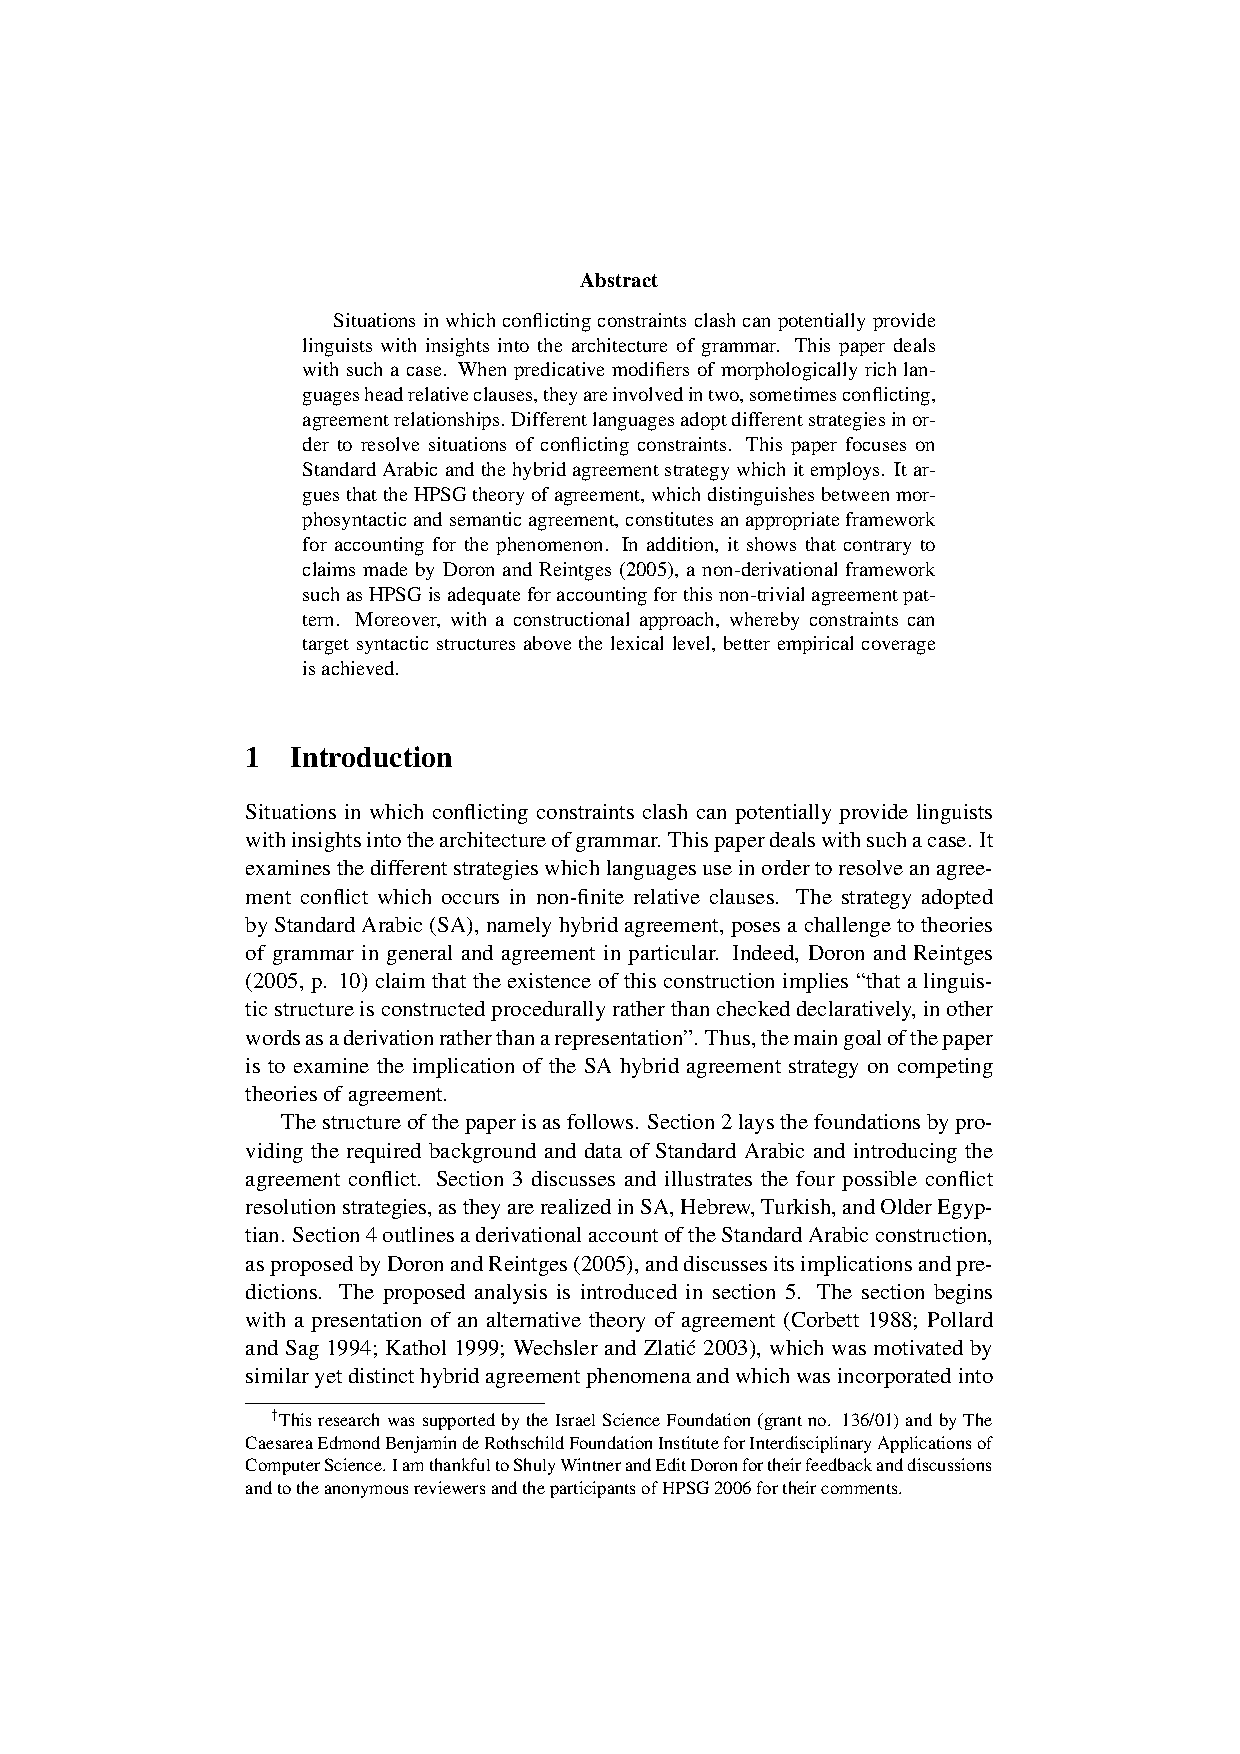
\includepdf[pages=-,pagecommand=\thispagestyle{plain}]{Includes/melnik.pdf}
        \setcounter{page}{247}
        \phantomsection
        \addcontentsline{toc}{section}{François Mouret: A Phrase Structure Approach to Argument Cluster Coordination}
\thispagestyle{empty}

\begin{center}
  {\huge\bfseries A Phrase Structure Approach to Argument Cluster Coordination\par}

  \bigskip

~\\
\begingroup
\setlength{\leftskip}{0pt plus 1fill}
\setlength{\rightskip}{0pt plus 1fill}
\setlength{\parindent}{0pt}
\setlength{\parfillskip}{0pt}
  \formatauthor{François Mouret}{\begin{tabular}{@{}c@{}}LLF, Université Paris 7-CNRS\end{tabular}}

\par\endgroup

  \vspace*{8ex}

  Proceedings of the 13th International Conference on\par Head-Driven Phrase Structure Grammar

  \bigskip

  Linguistic Modelling Laboratory,\\Institute for Parallel Processing,\\Bulgarian Academy of Sciences,\\Sofia,\\Held in Varna

  \medskip

  Stefan Müller (Editor)

  \medskip

  2006

  \medskip

  CSLI Publications

  \medskip

  pages 247--267

  \medskip

  \url{http://csli-publications.stanford.edu/HPSG/2006}
\end{center}
\vfill

\noindent



\vfill
\noindent
% APA Style
Mouret, François. 2006. A Phrase Structure Approach to Argument Cluster Coordination. In Müller, Stefan (Ed.), \emph{{Proceedings of the 13th International Conference on Head-Driven Phrase Structure Grammar, Varna}}, 247--267. Stanford,
CA: CSLI Publications. \hfill\href{http://creativecommons.org/licenses/by/4.0/}{\includegraphics[height=.75em]{Includes/ccby.eps}}

\newpage
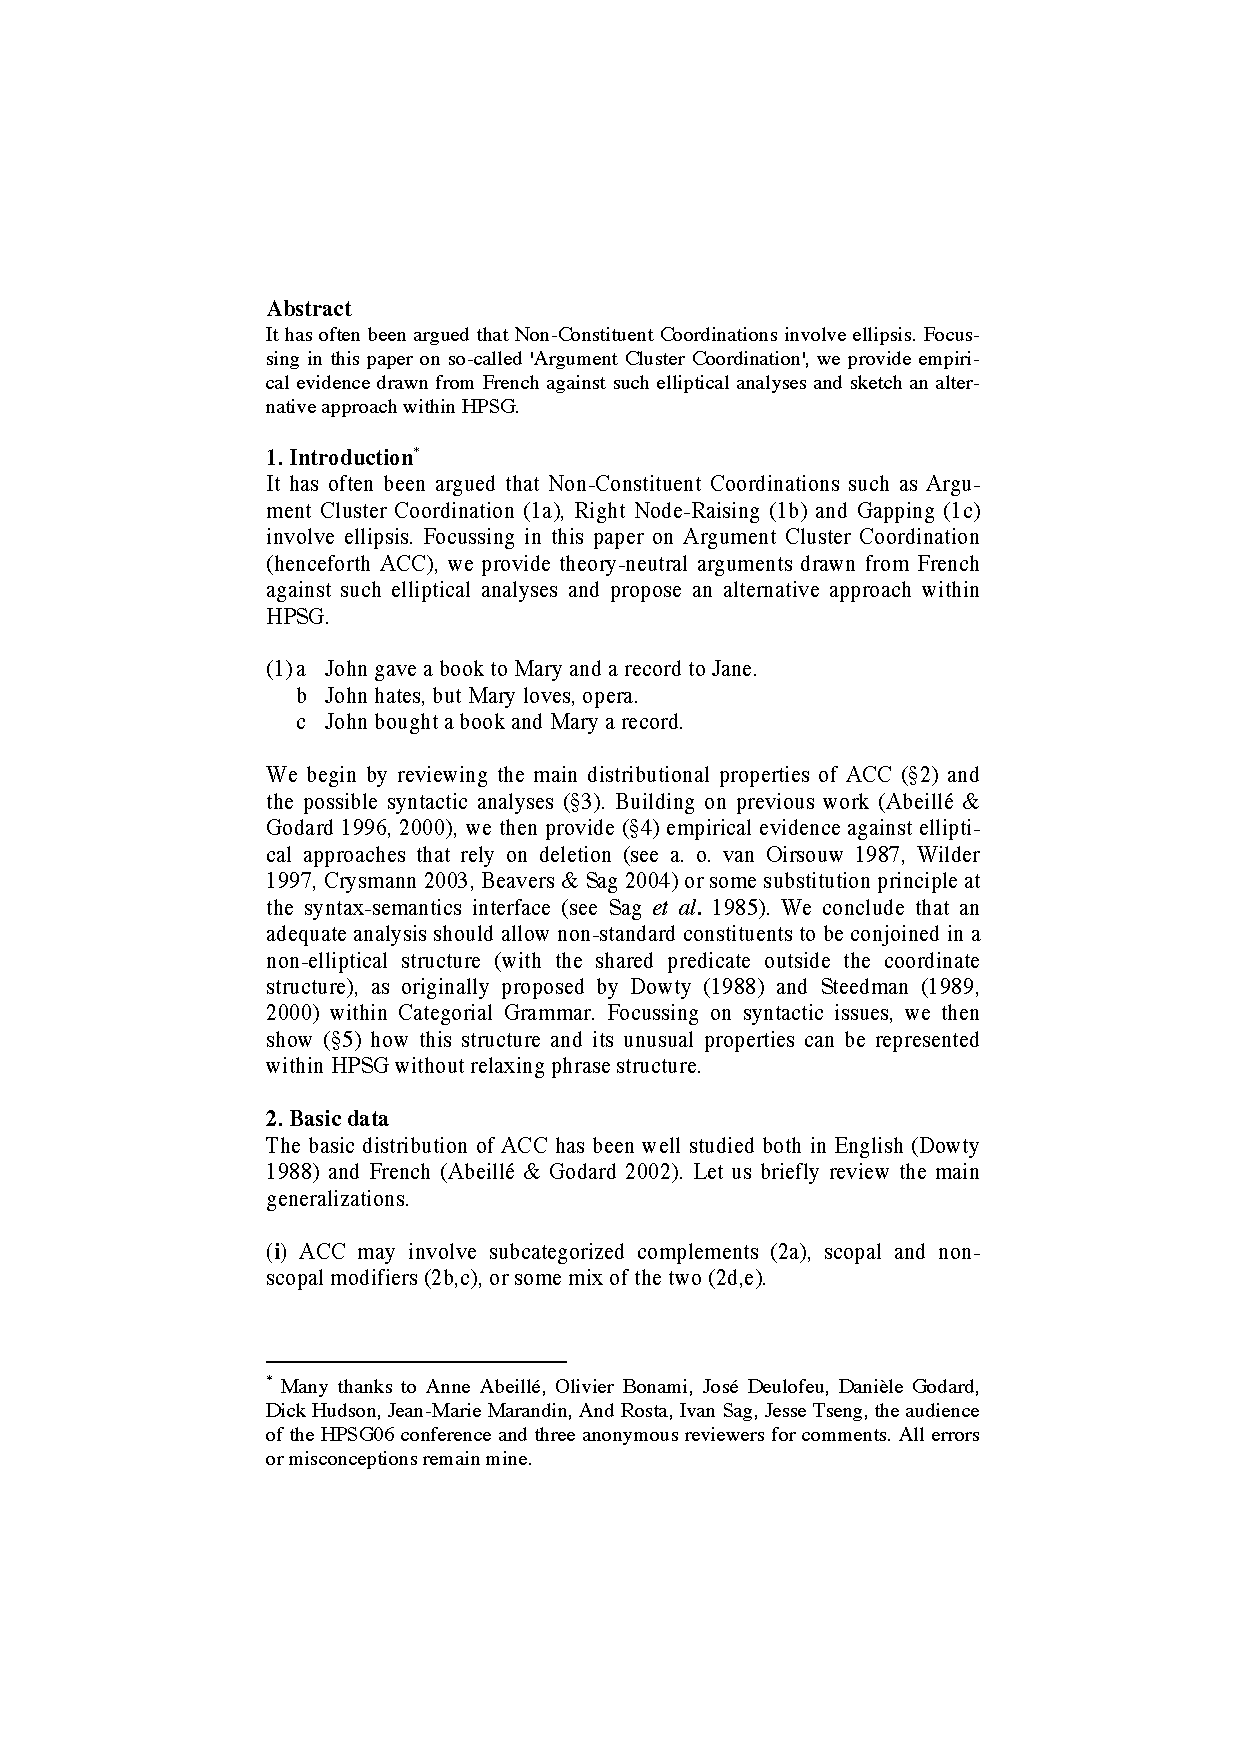
\includepdf[pages=-,pagecommand=\thispagestyle{plain}]{Includes/mouret.pdf}
        \setcounter{page}{268}
        \phantomsection
        \addcontentsline{toc}{section}{Katsuaki Nakanishi: A Unified Approach to Questions, Quantifiers, and
Coordination in Japanese}
\thispagestyle{empty}

\begin{center}
  {\huge\bfseries A Unified Approach to Questions, Quantifiers, and
Coordination in Japanese\par}

  \bigskip

~\\
\begingroup
\setlength{\leftskip}{0pt plus 1fill}
\setlength{\rightskip}{0pt plus 1fill}
\setlength{\parindent}{0pt}
\setlength{\parfillskip}{0pt}
  \formatauthor{Katsuaki Nakanishi}{\begin{tabular}{@{}c@{}}Department of Language and Information Sciences University of Tokyo\end{tabular}}

\par\endgroup

  \vspace*{8ex}

  Proceedings of the 13th International Conference on\par Head-Driven Phrase Structure Grammar

  \bigskip

  Linguistic Modelling Laboratory,\\Institute for Parallel Processing,\\Bulgarian Academy of Sciences,\\Sofia,\\Held in Varna

  \medskip

  Stefan Müller (Editor)

  \medskip

  2006

  \medskip

  CSLI Publications

  \medskip

  pages 268--283

  \medskip

  \url{http://csli-publications.stanford.edu/HPSG/2006}
\end{center}
\vfill

\noindent



\vfill
\noindent
% APA Style
Nakanishi, Katsuaki. 2006. A Unified Approach to Questions, Quantifiers, and
Coordination in Japanese. In Müller, Stefan (Ed.), \emph{{Proceedings of the 13th International Conference on Head-Driven Phrase Structure Grammar, Varna}}, 268--283. Stanford,
CA: CSLI Publications. \hfill\href{http://creativecommons.org/licenses/by/4.0/}{\includegraphics[height=.75em]{Includes/ccby.eps}}

\newpage
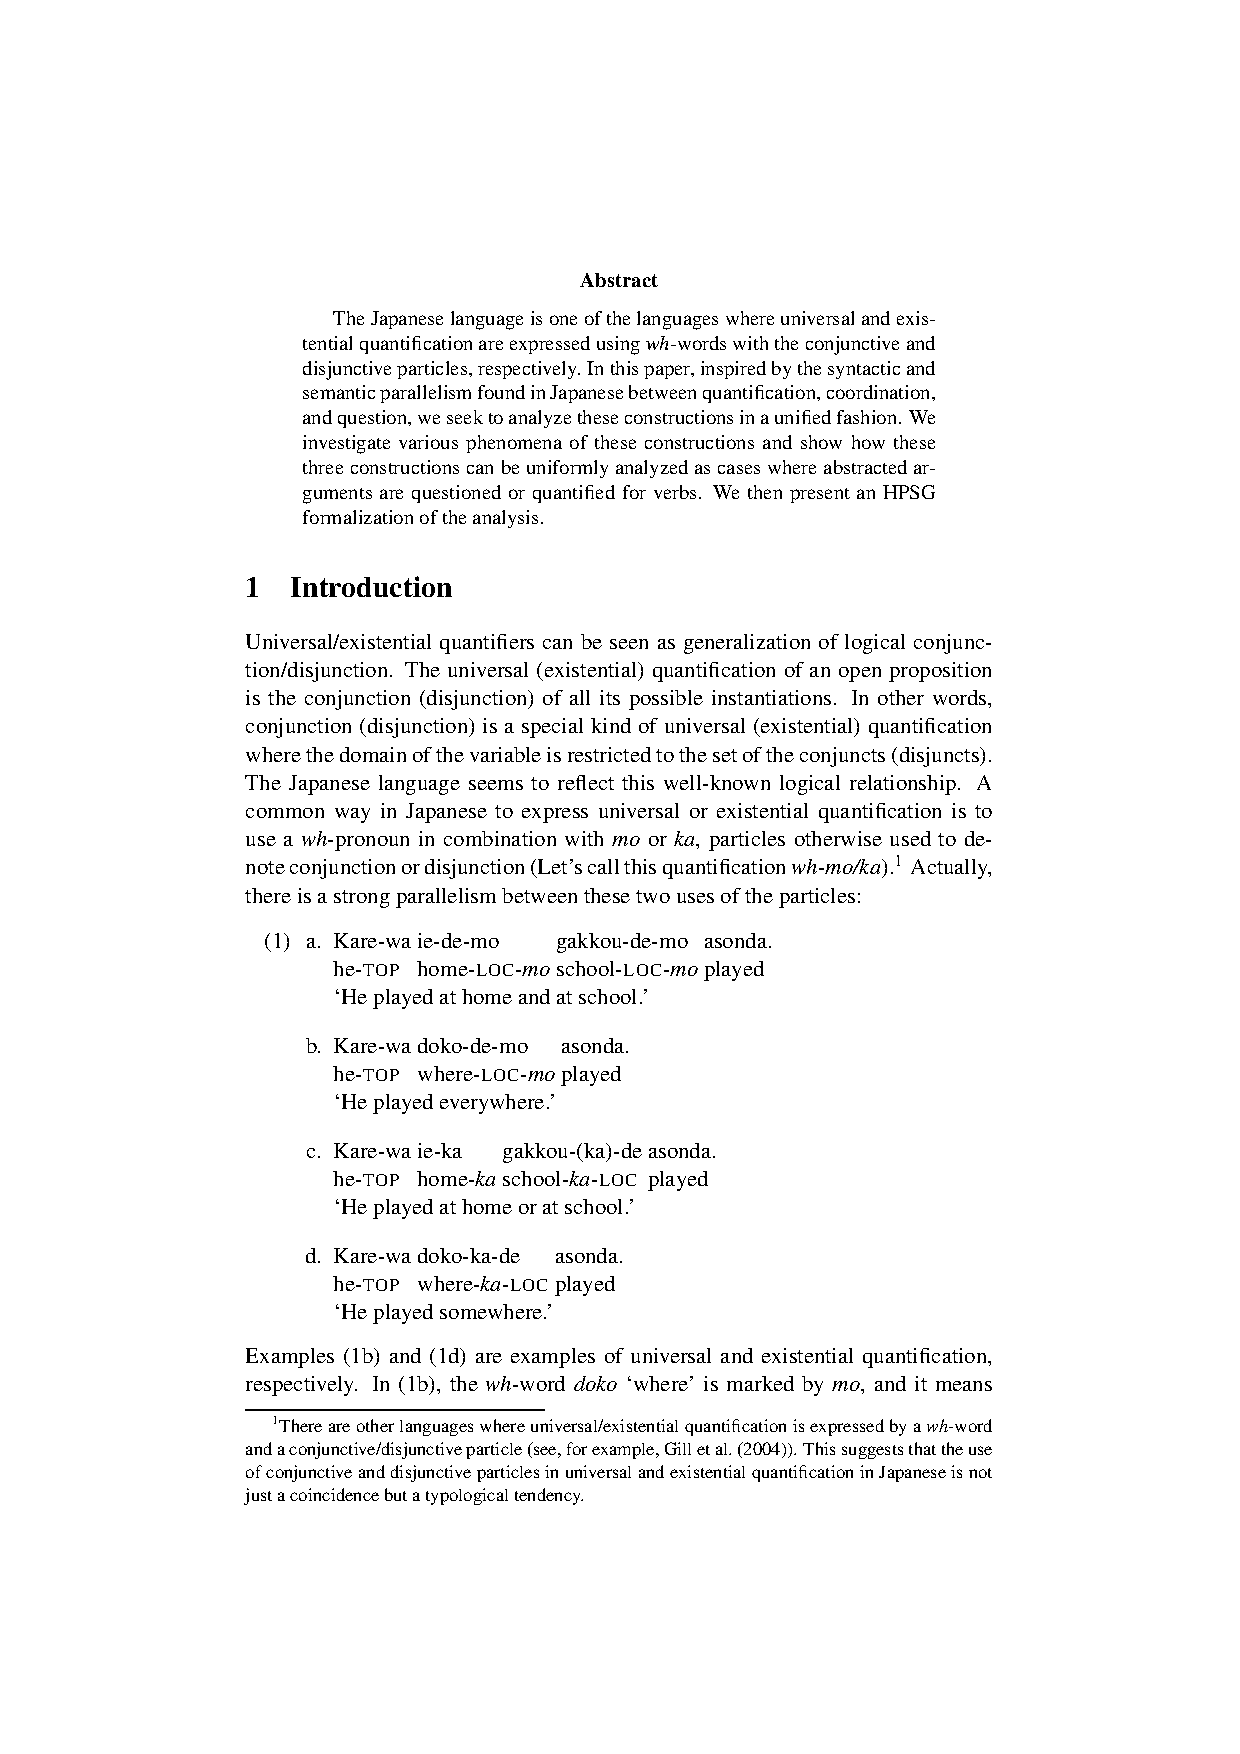
\includepdf[pages=-,pagecommand=\thispagestyle{plain}]{Includes/nakanishi.pdf}
        \setcounter{page}{284}
        \phantomsection
        \addcontentsline{toc}{section}{Tsuneko Nakazawa: Motion Event and Deictic Motion Verbs as Path-Conflating Verbs}
\thispagestyle{empty}

\begin{center}
  {\huge\bfseries Motion Event and Deictic Motion Verbs as Path-Conflating Verbs\par}

  \bigskip

~\\
\begingroup
\setlength{\leftskip}{0pt plus 1fill}
\setlength{\rightskip}{0pt plus 1fill}
\setlength{\parindent}{0pt}
\setlength{\parfillskip}{0pt}
  \formatauthor{Tsuneko Nakazawa}{\begin{tabular}{@{}c@{}}University of Tokyo\end{tabular}}

\par\endgroup

  \vspace*{8ex}

  Proceedings of the 13th International Conference on\par Head-Driven Phrase Structure Grammar

  \bigskip

  Linguistic Modelling Laboratory,\\Institute for Parallel Processing,\\Bulgarian Academy of Sciences,\\Sofia,\\Held in Varna

  \medskip

  Stefan Müller (Editor)

  \medskip

  2006

  \medskip

  CSLI Publications

  \medskip

  pages 284--304

  \medskip

  \url{http://csli-publications.stanford.edu/HPSG/2006}
\end{center}
\vfill

\noindent



\vfill
\noindent
% APA Style
Nakazawa, Tsuneko. 2006. Motion Event and Deictic Motion Verbs as Path-Conflating Verbs. In Müller, Stefan (Ed.), \emph{{Proceedings of the 13th International Conference on Head-Driven Phrase Structure Grammar, Varna}}, 284--304. Stanford,
CA: CSLI Publications. \hfill\href{http://creativecommons.org/licenses/by/4.0/}{\includegraphics[height=.75em]{Includes/ccby.eps}}

\newpage
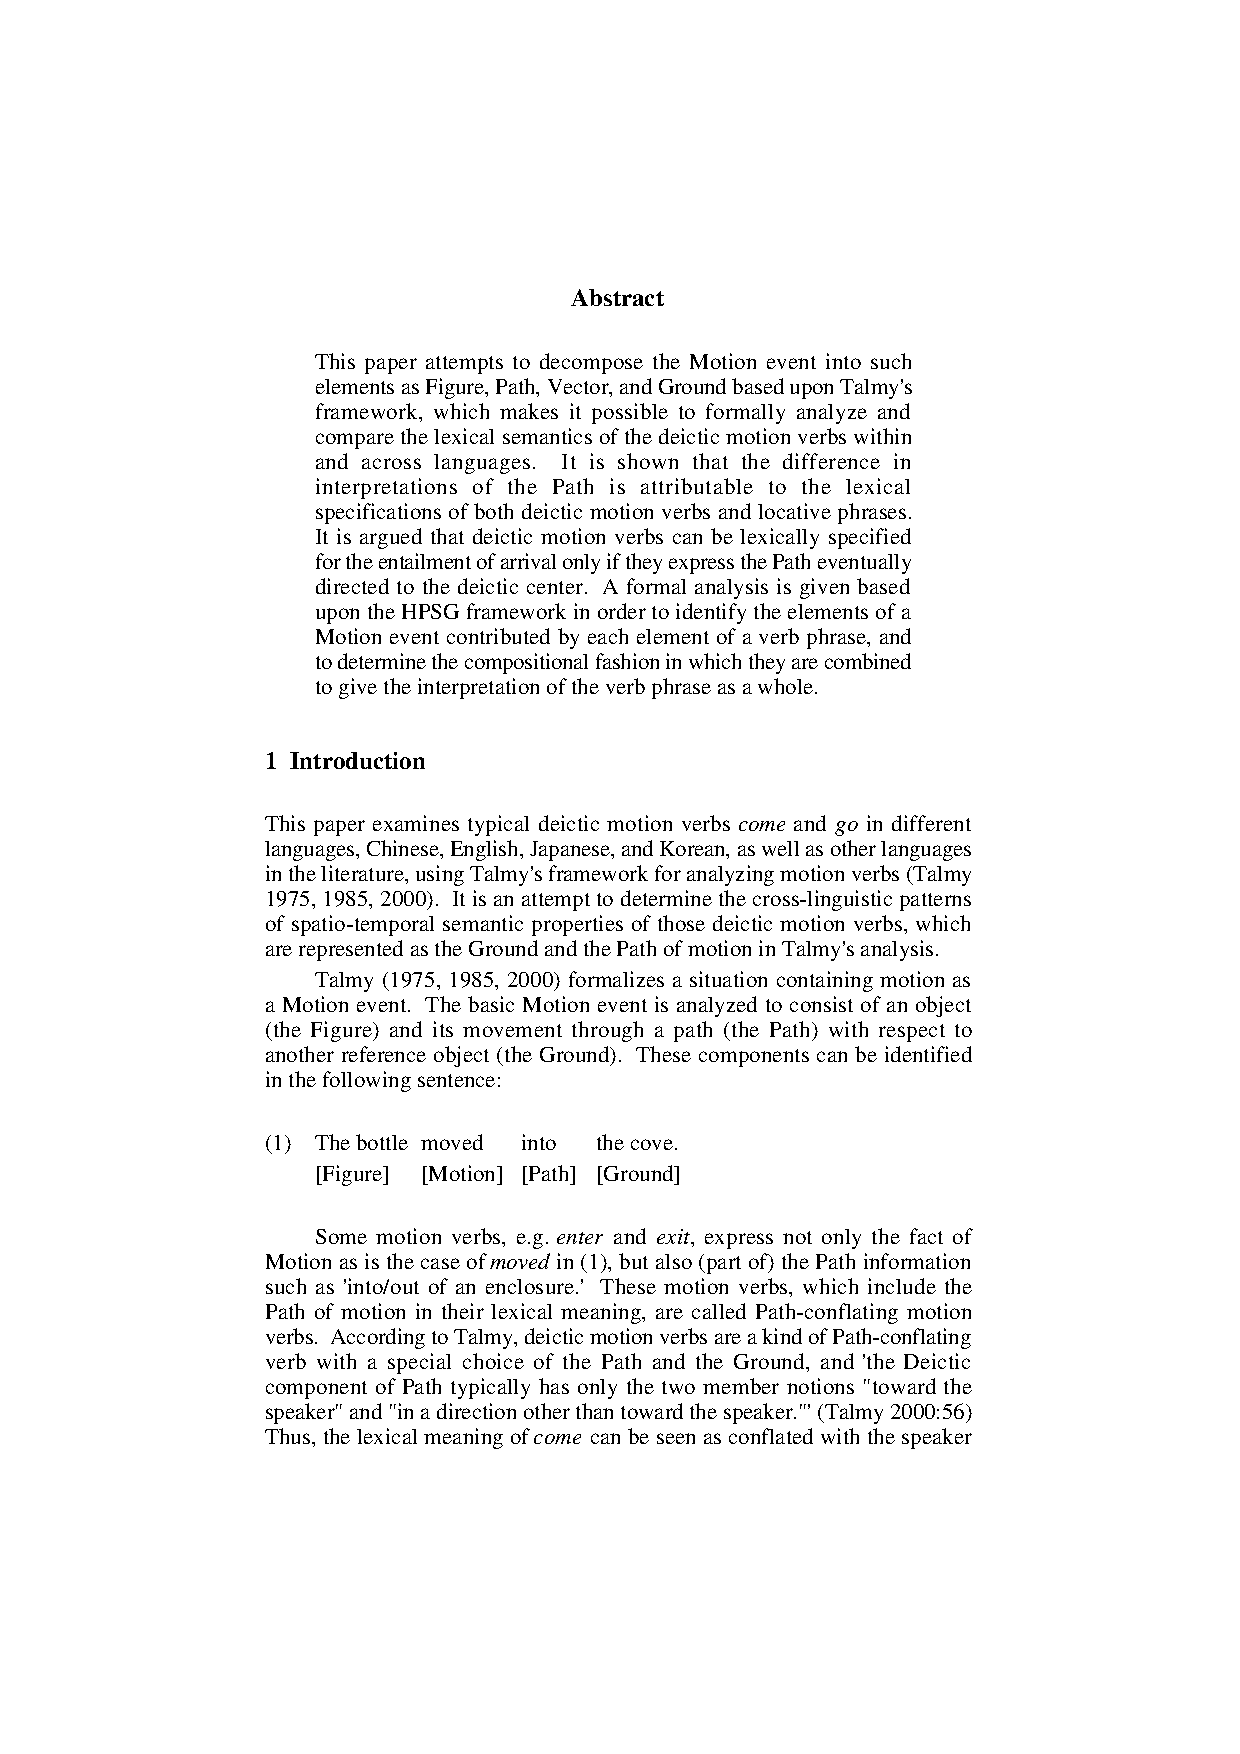
\includepdf[pages=-,pagecommand=\thispagestyle{plain}]{Includes/nakazawa.pdf}
        \setcounter{page}{305}
        \phantomsection
        \addcontentsline{toc}{section}{Frank Richter, Manfred Sailer: Modeling Typological Markedness in Semantics: The Case of Negative Concord}
\thispagestyle{empty}

\begin{center}
  {\huge\bfseries Modeling Typological Markedness in Semantics: The Case of Negative Concord\par}

  \bigskip

~\\
\begingroup
\setlength{\leftskip}{0pt plus 1fill}
\setlength{\rightskip}{0pt plus 1fill}
\setlength{\parindent}{0pt}
\setlength{\parfillskip}{0pt}
  \formatauthor{Frank Richter}{\begin{tabular}{@{}c@{}}University of Tübingen\end{tabular}}
\formatauthor{Manfred Sailer}{\begin{tabular}{@{}c@{}}University of Göttingen\end{tabular}}

\par\endgroup

  \vspace*{8ex}

  Proceedings of the 13th International Conference on\par Head-Driven Phrase Structure Grammar

  \bigskip

  Linguistic Modelling Laboratory,\\Institute for Parallel Processing,\\Bulgarian Academy of Sciences,\\Sofia,\\Held in Varna

  \medskip

  Stefan Müller (Editor)

  \medskip

  2006

  \medskip

  CSLI Publications

  \medskip

  pages 305--325

  \medskip

  \url{http://csli-publications.stanford.edu/HPSG/2006}
\end{center}
\vfill

\noindent



\vfill
\noindent
% APA Style
Richter, Frank, \& Sailer, Manfred. 2006. Modeling Typological Markedness in Semantics: The Case of Negative Concord. In Müller, Stefan (Ed.), \emph{{Proceedings of the 13th International Conference on Head-Driven Phrase Structure Grammar, Varna}}, 305--325. Stanford,
CA: CSLI Publications. \hfill\href{http://creativecommons.org/licenses/by/4.0/}{\includegraphics[height=.75em]{Includes/ccby.eps}}

\newpage
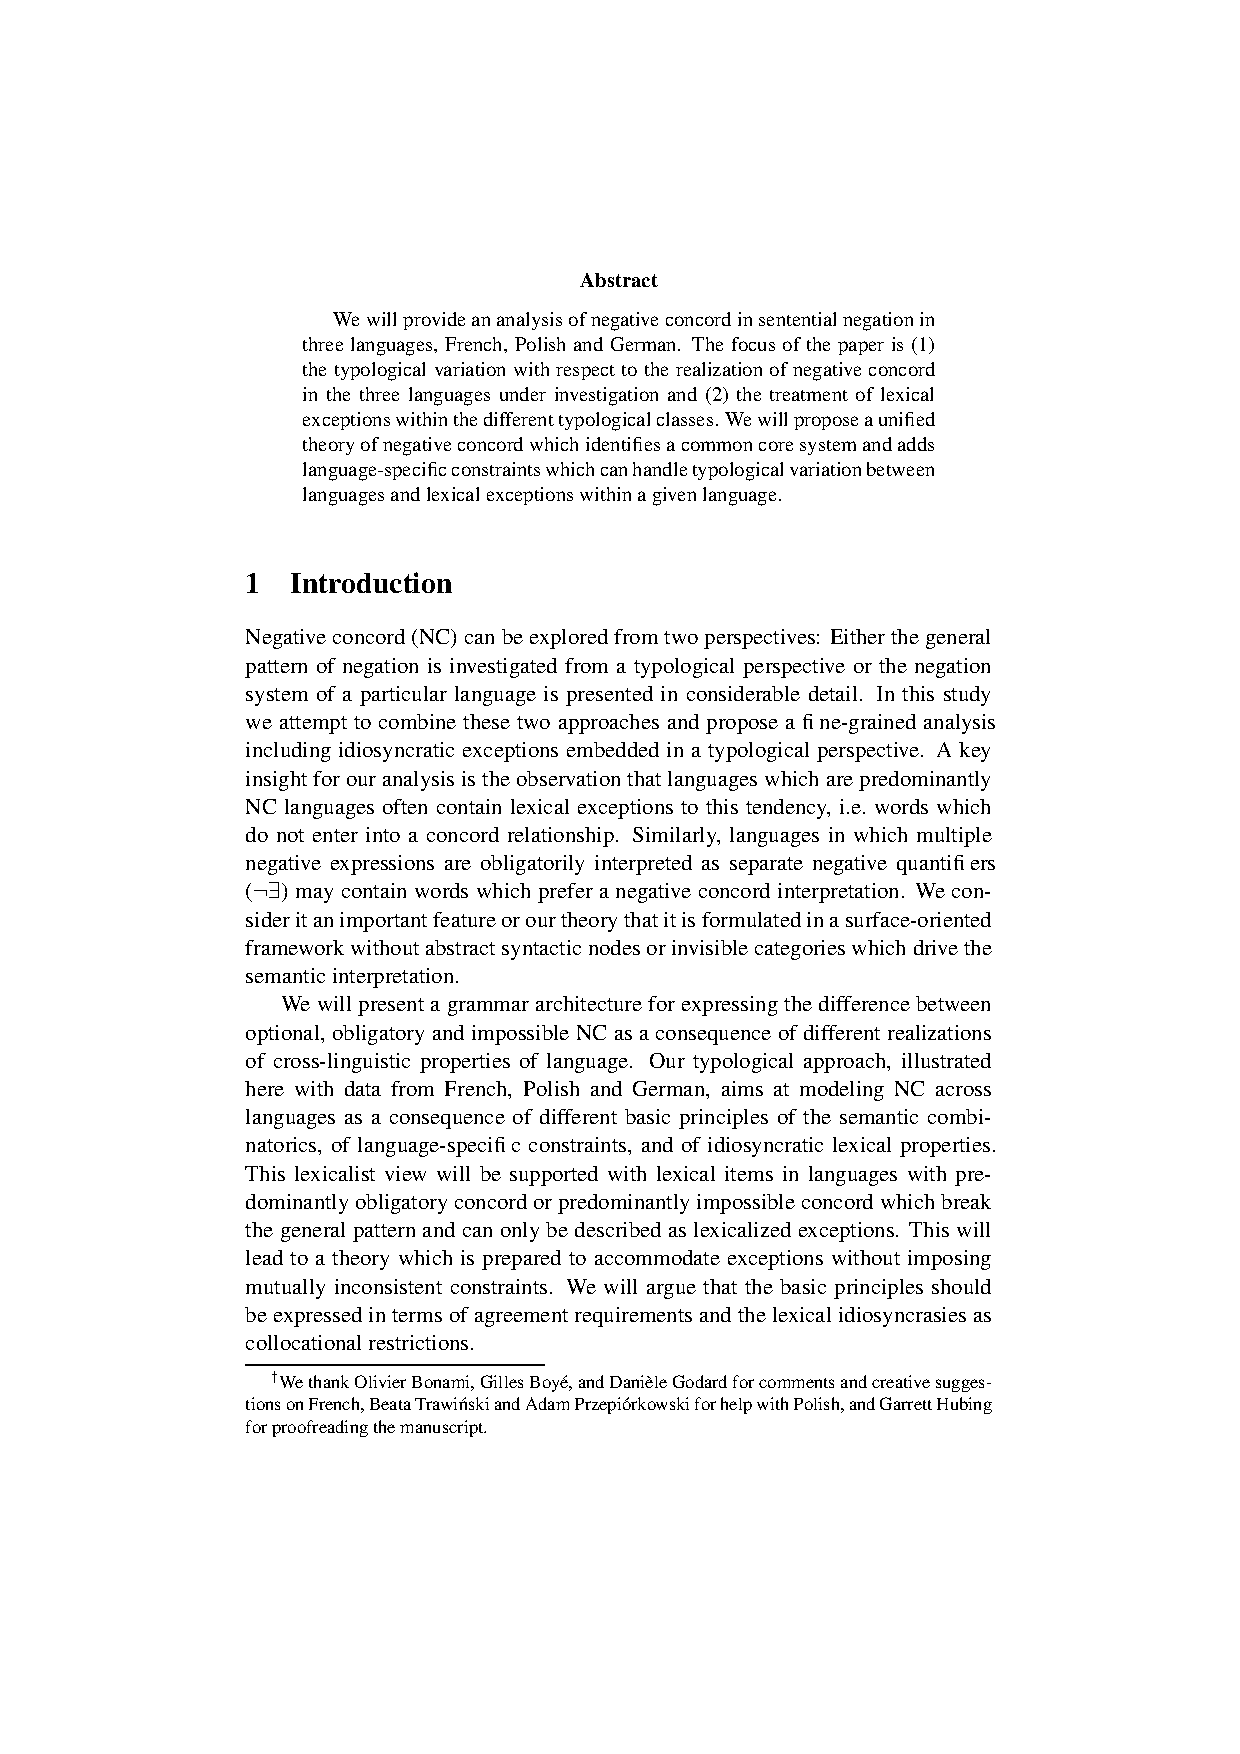
\includepdf[pages=-,pagecommand=\thispagestyle{plain}]{Includes/richter-sailer.pdf}
        \setcounter{page}{326}
        \phantomsection
        \addcontentsline{toc}{section}{Yo Sato: A Proposed Lexicalised Linearisation Grammar -- a monostratal alternative}
\thispagestyle{empty}

\begin{center}
  {\huge\bfseries A Proposed Lexicalised Linearisation Grammar -- a monostratal alternative\par}

  \bigskip

~\\
\begingroup
\setlength{\leftskip}{0pt plus 1fill}
\setlength{\rightskip}{0pt plus 1fill}
\setlength{\parindent}{0pt}
\setlength{\parfillskip}{0pt}
  \formatauthor{Yo Sato}{\begin{tabular}{@{}c@{}}Department of Computer Science King's College London\end{tabular}}

\par\endgroup

  \vspace*{8ex}

  Proceedings of the 13th International Conference on\par Head-Driven Phrase Structure Grammar

  \bigskip

  Linguistic Modelling Laboratory,\\Institute for Parallel Processing,\\Bulgarian Academy of Sciences,\\Sofia,\\Held in Varna

  \medskip

  Stefan Müller (Editor)

  \medskip

  2006

  \medskip

  CSLI Publications

  \medskip

  pages 326--338

  \medskip

  \url{http://csli-publications.stanford.edu/HPSG/2006}
\end{center}
\vfill

\noindent



\vfill
\noindent
% APA Style
Sato, Yo. 2006. A Proposed Lexicalised Linearisation Grammar -- a monostratal alternative. In Müller, Stefan (Ed.), \emph{{Proceedings of the 13th International Conference on Head-Driven Phrase Structure Grammar, Varna}}, 326--338. Stanford,
CA: CSLI Publications. \hfill\href{http://creativecommons.org/licenses/by/4.0/}{\includegraphics[height=.75em]{Includes/ccby.eps}}

\newpage
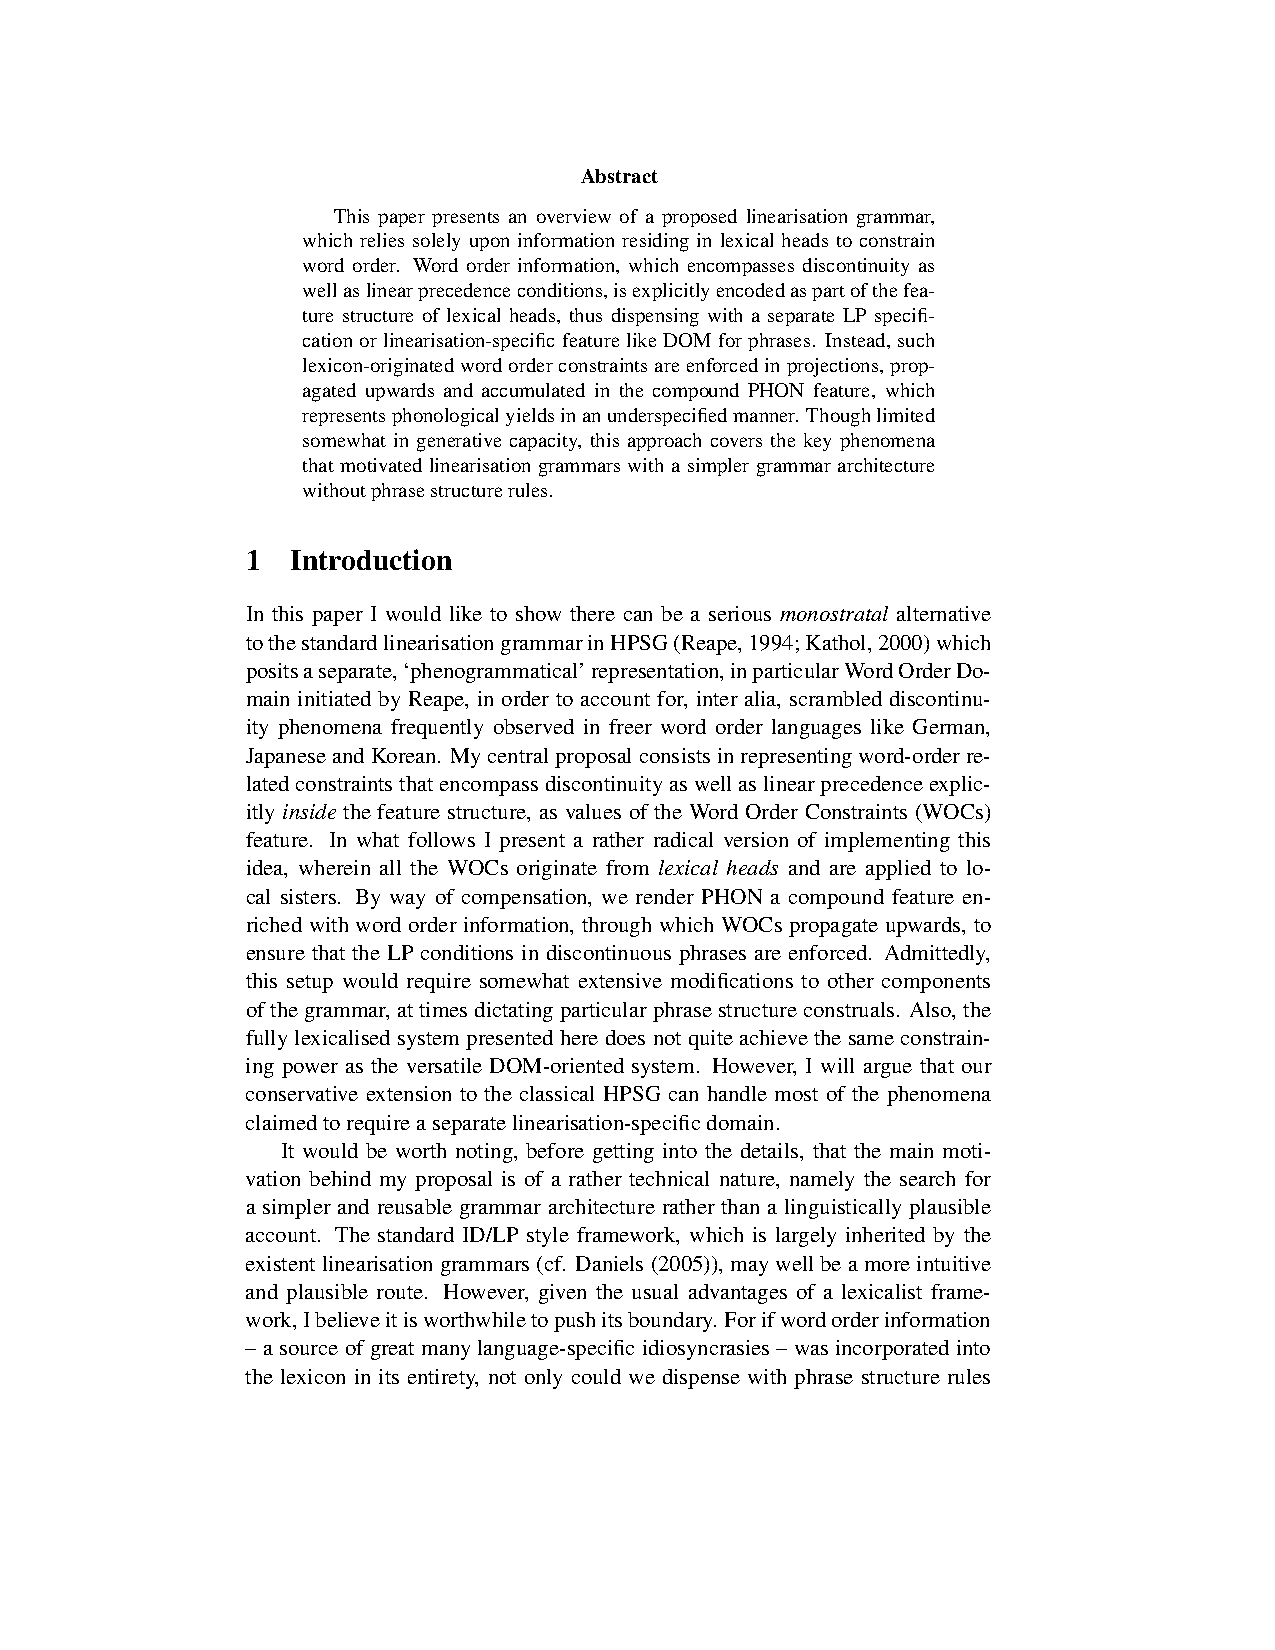
\includepdf[pages=-,pagecommand=\thispagestyle{plain}]{Includes/sato.pdf}
        \setcounter{page}{339}
        \phantomsection
        \addcontentsline{toc}{section}{Harry J. Tily, Ivan A. Sag: A Unified Analysis of French Causatives}
\thispagestyle{empty}

\begin{center}
  {\huge\bfseries A Unified Analysis of French Causatives\par}

  \bigskip

~\\
\begingroup
\setlength{\leftskip}{0pt plus 1fill}
\setlength{\rightskip}{0pt plus 1fill}
\setlength{\parindent}{0pt}
\setlength{\parfillskip}{0pt}
  \formatauthor{Harry J. Tily}{\begin{tabular}{@{}c@{}}Department of Linguistics, Stanford University\end{tabular}}
\formatauthor{Ivan A. Sag}{\begin{tabular}{@{}c@{}}Department of Linguistics, Stanford University\end{tabular}}

\par\endgroup

  \vspace*{8ex}

  Proceedings of the 13th International Conference on\par Head-Driven Phrase Structure Grammar

  \bigskip

  Linguistic Modelling Laboratory,\\Institute for Parallel Processing,\\Bulgarian Academy of Sciences,\\Sofia,\\Held in Varna

  \medskip

  Stefan Müller (Editor)

  \medskip

  2006

  \medskip

  CSLI Publications

  \medskip

  pages 339--359

  \medskip

  \url{http://csli-publications.stanford.edu/HPSG/2006}
\end{center}
\vfill

\noindent



\vfill
\noindent
% APA Style
Tily, Harry J., \& Sag, Ivan A. 2006. A Unified Analysis of French Causatives. In Müller, Stefan (Ed.), \emph{{Proceedings of the 13th International Conference on Head-Driven Phrase Structure Grammar, Varna}}, 339--359. Stanford,
CA: CSLI Publications. \hfill\href{http://creativecommons.org/licenses/by/4.0/}{\includegraphics[height=.75em]{Includes/ccby.eps}}

\newpage
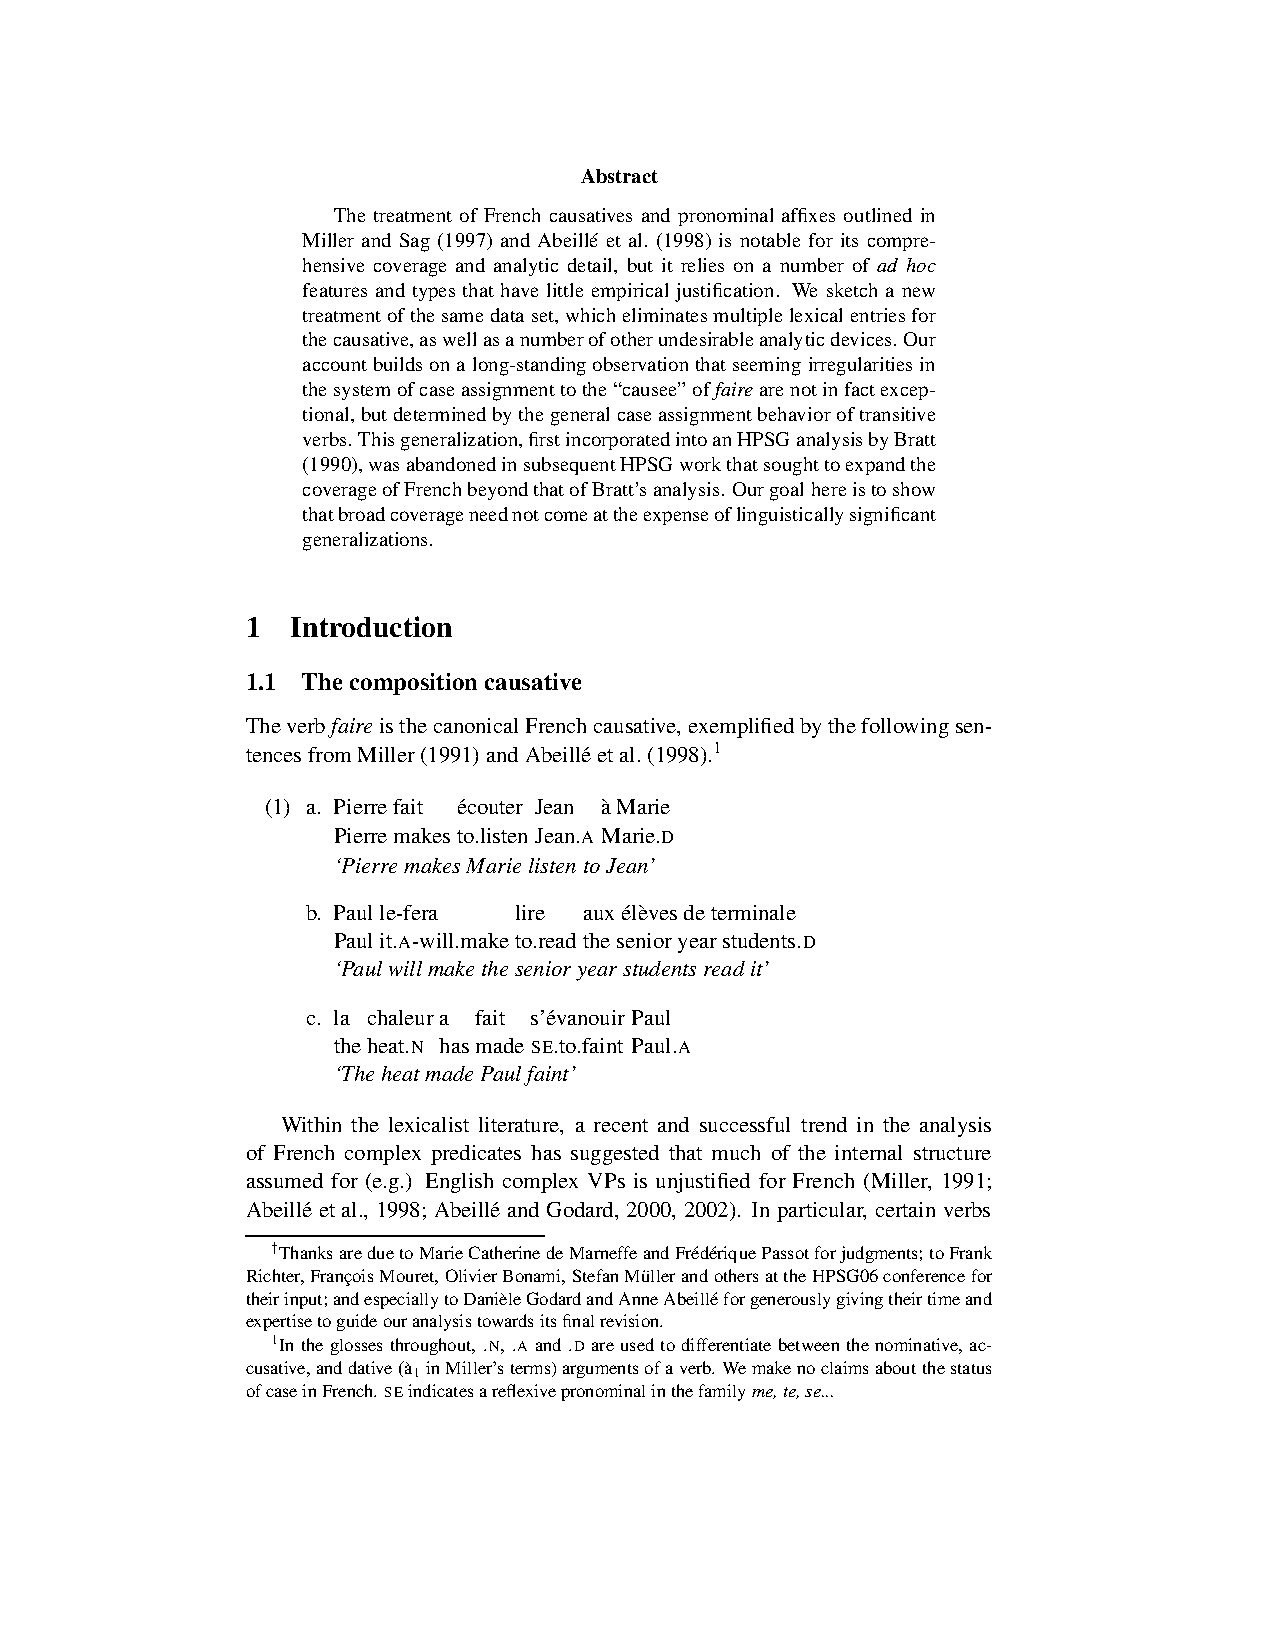
\includepdf[pages=-,pagecommand=\thispagestyle{plain}]{Includes/tily-sag.pdf}
\part{Contributions to the Workshop}
\thispagestyle{empty}
\newpage
        \setcounter{page}{361}
        \phantomsection
        \addcontentsline{toc}{section}{Olivier Bonami, Gilles Boy{\'e}: Deriving Inflectional Irregularity}
\thispagestyle{empty}

\begin{center}
  {\huge\bfseries Deriving Inflectional Irregularity\par}

  \bigskip

~\\
\begingroup
\setlength{\leftskip}{0pt plus 1fill}
\setlength{\rightskip}{0pt plus 1fill}
\setlength{\parindent}{0pt}
\setlength{\parfillskip}{0pt}
  \formatauthor{Olivier Bonami}{\begin{tabular}{@{}c@{}}Université Paris-Sorbonne\end{tabular}}
\formatauthor{Gilles Boyé}{\begin{tabular}{@{}c@{}}LLF\end{tabular}}

\par\endgroup

  \vspace*{8ex}

  Proceedings of the 13th International Conference on\par Head-Driven Phrase Structure Grammar

  \bigskip

  Linguistic Modelling Laboratory,\\Institute for Parallel Processing,\\Bulgarian Academy of Sciences,\\Sofia,\\Held in Varna

  \medskip

  Stefan Müller (Editor)

  \medskip

  2006

  \medskip

  CSLI Publications

  \medskip

  pages 361--380

  \medskip

  \url{http://csli-publications.stanford.edu/HPSG/2006}
\end{center}
\vfill

\noindent



\vfill
\noindent
% APA Style
Bonami, Olivier, \& Boyé,  Gilles. 2006. Deriving Inflectional Irregularity. In Müller, Stefan (Ed.), \emph{{Proceedings of the 13th International Conference on Head-Driven Phrase Structure Grammar, Varna}}, 361--380. Stanford,
CA: CSLI Publications. \hfill\href{http://creativecommons.org/licenses/by/4.0/}{\includegraphics[height=.75em]{Includes/ccby.eps}}

\newpage
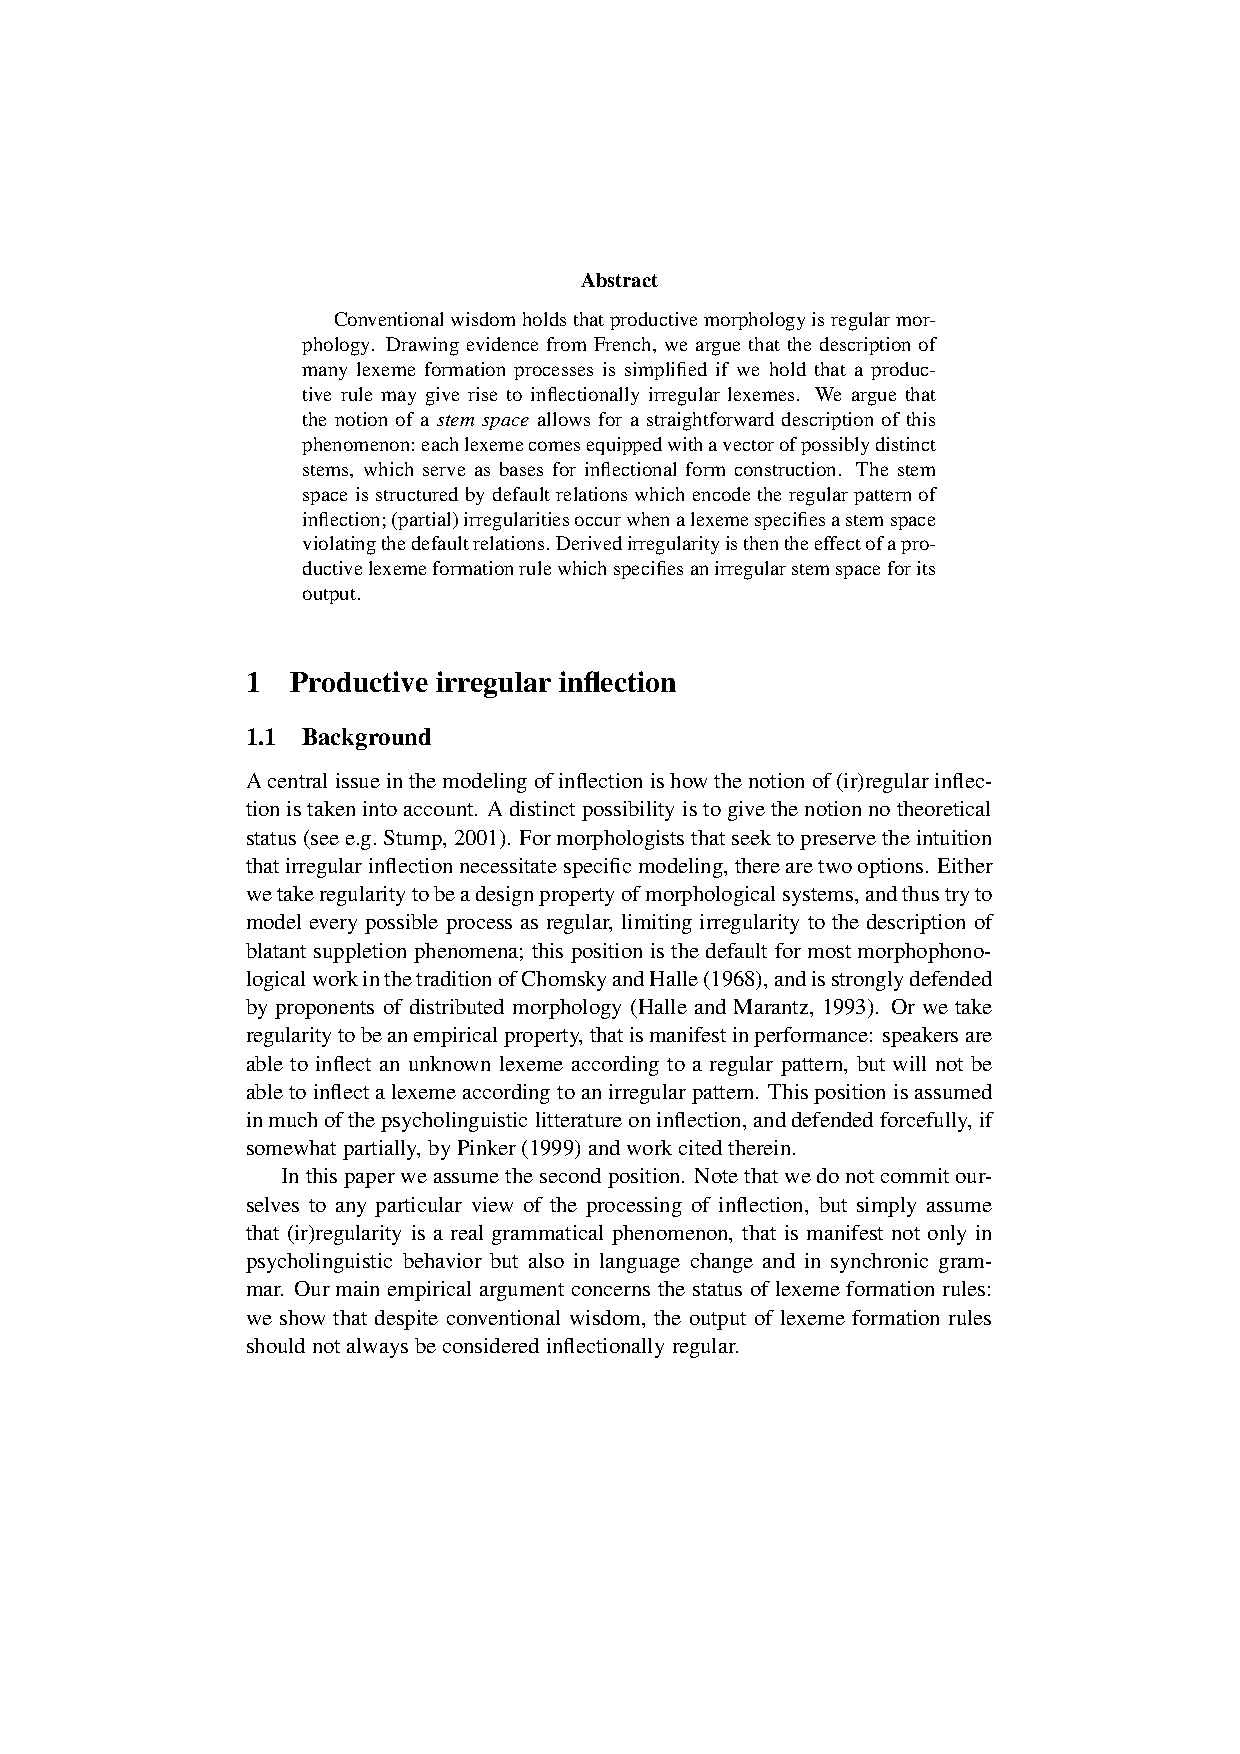
\includepdf[pages=-,pagecommand=\thispagestyle{plain}]{Includes/bonami-boye.pdf}
        \setcounter{page}{381}
        \phantomsection
        \addcontentsline{toc}{section}{Jonathan Allen Brindle: Uncovering regularities: On Bare and Evaluated Controllers in Tigrinya}
\thispagestyle{empty}

\begin{center}
  {\huge\bfseries Uncovering regularities: On Bare and Evaluated Controllers in Tigrinya\par}

  \bigskip

~\\
\begingroup
\setlength{\leftskip}{0pt plus 1fill}
\setlength{\rightskip}{0pt plus 1fill}
\setlength{\parindent}{0pt}
\setlength{\parfillskip}{0pt}
  \formatauthor{Jonathan Allen Brindle}{\begin{tabular}{@{}c@{}}Norges Teknisk-Naturvitenskapelige Universitet\end{tabular}}

\par\endgroup

  \vspace*{8ex}

  Proceedings of the 13th International Conference on\par Head-Driven Phrase Structure Grammar

  \bigskip

  Linguistic Modelling Laboratory,\\Institute for Parallel Processing,\\Bulgarian Academy of Sciences,\\Sofia,\\Held in Varna

  \medskip

  Stefan Müller (Editor)

  \medskip

  2006

  \medskip

  CSLI Publications

  \medskip

  pages 381--401

  \medskip

  \url{http://csli-publications.stanford.edu/HPSG/2006}
\end{center}
\vfill

\noindent



\vfill
\noindent
% APA Style
Brindle, Jonathan Allen. 2006. Uncovering regularities: On Bare and Evaluated Controllers in Tigrinya. In Müller, Stefan (Ed.), \emph{{Proceedings of the 13th International Conference on Head-Driven Phrase Structure Grammar, Varna}}, 381--401. Stanford,
CA: CSLI Publications. \hfill\href{http://creativecommons.org/licenses/by/4.0/}{\includegraphics[height=.75em]{Includes/ccby.eps}}

\newpage
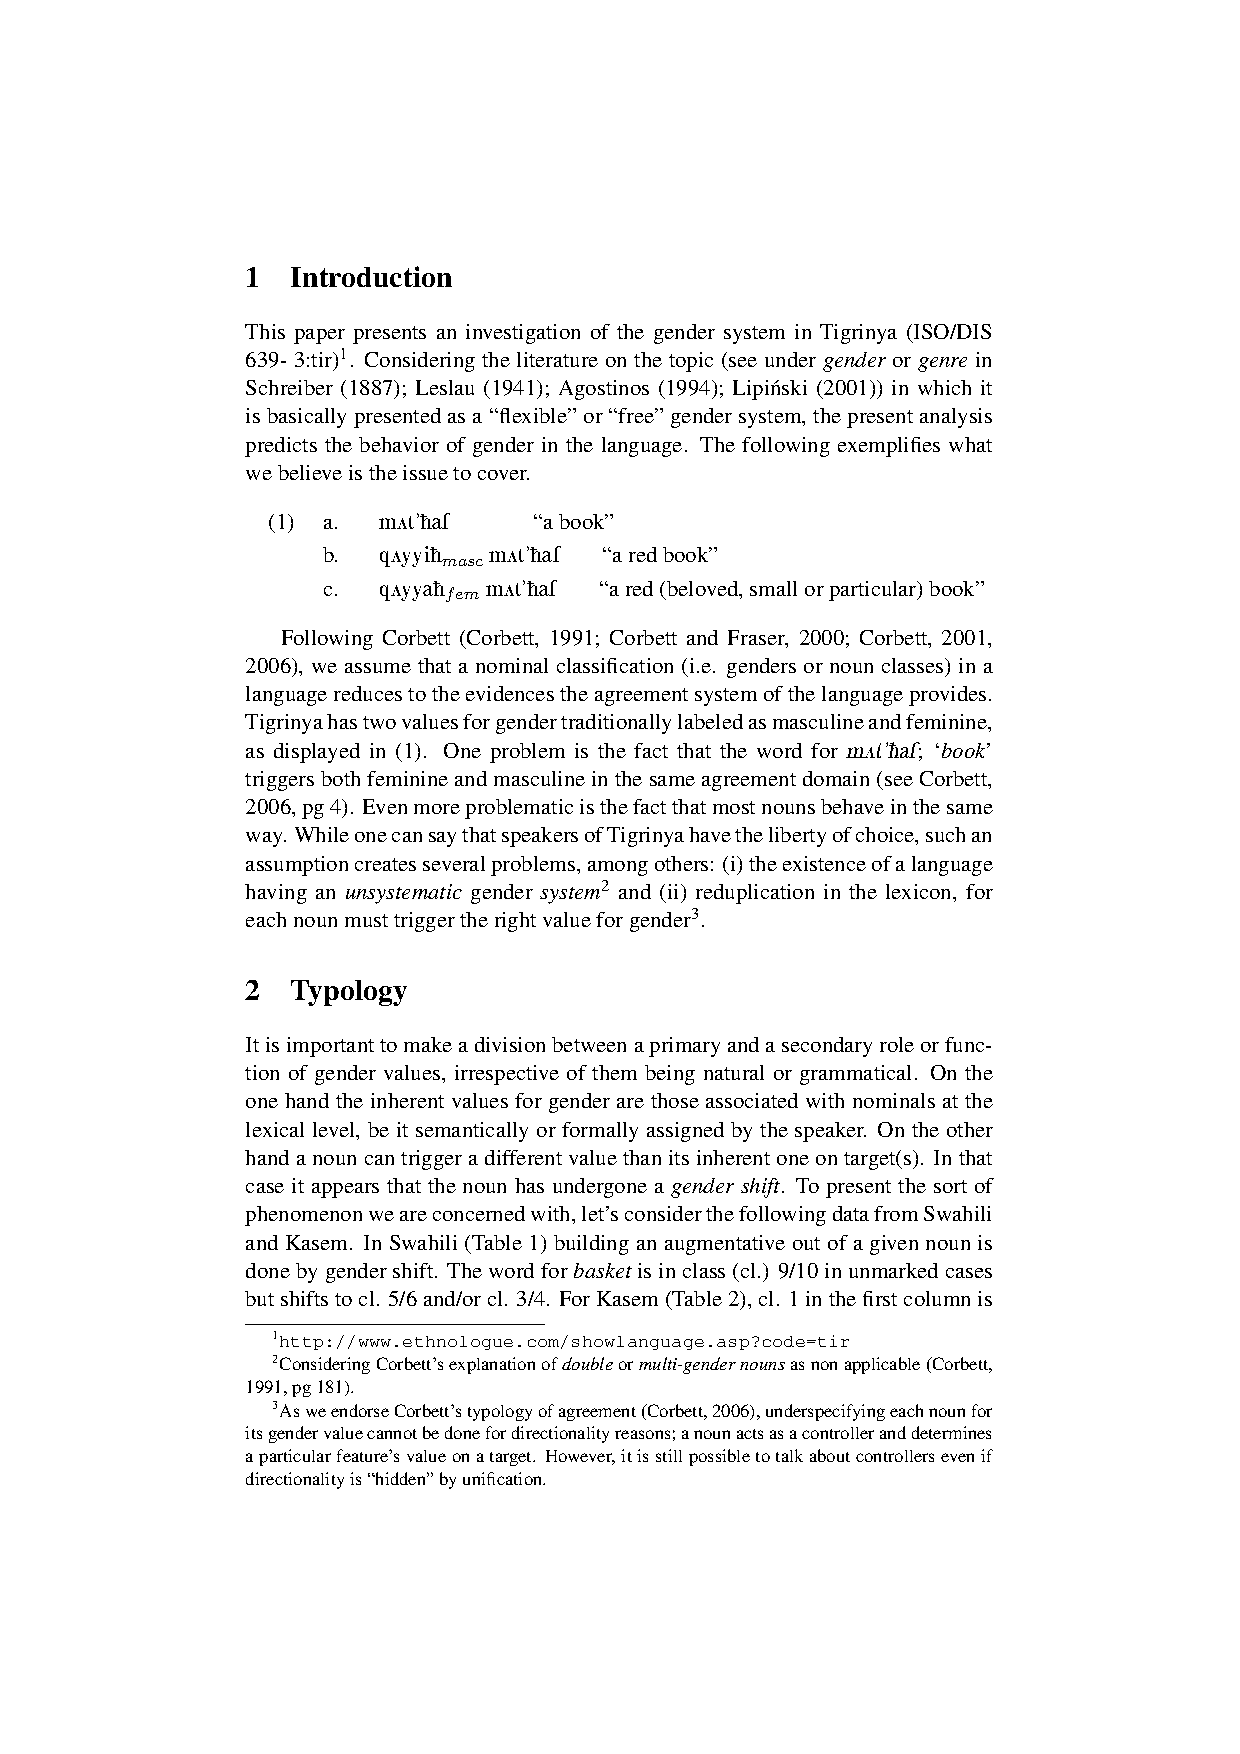
\includepdf[pages=-,pagecommand=\thispagestyle{plain}]{Includes/brindle.pdf}
        \setcounter{page}{402}
        \phantomsection
        \addcontentsline{toc}{section}{Hyun-Jong Hahm: Number Agreement in Russian Predicates}
\thispagestyle{empty}

\begin{center}
  {\huge\bfseries Number Agreement in Russian Predicates\par}

  \bigskip

~\\
\begingroup
\setlength{\leftskip}{0pt plus 1fill}
\setlength{\rightskip}{0pt plus 1fill}
\setlength{\parindent}{0pt}
\setlength{\parfillskip}{0pt}
  \formatauthor{Hyun-Jong Hahm}{\begin{tabular}{@{}c@{}}The University of Texas at Austin\end{tabular}}

\par\endgroup

  \vspace*{8ex}

  Proceedings of the 13th International Conference on\par Head-Driven Phrase Structure Grammar

  \bigskip

  Linguistic Modelling Laboratory,\\Institute for Parallel Processing,\\Bulgarian Academy of Sciences,\\Sofia,\\Held in Varna

  \medskip

  Stefan Müller (Editor)

  \medskip

  2006

  \medskip

  CSLI Publications

  \medskip

  pages 402--420

  \medskip

  \url{http://csli-publications.stanford.edu/HPSG/2006}
\end{center}
\vfill

\noindent



\vfill
\noindent
% APA Style
Hahm, Hyun-Jong. 2006. Number Agreement in Russian Predicates. In Müller, Stefan (Ed.), \emph{{Proceedings of the 13th International Conference on Head-Driven Phrase Structure Grammar, Varna}}, 402--420. Stanford,
CA: CSLI Publications. \hfill\href{http://creativecommons.org/licenses/by/4.0/}{\includegraphics[height=.75em]{Includes/ccby.eps}}

\newpage
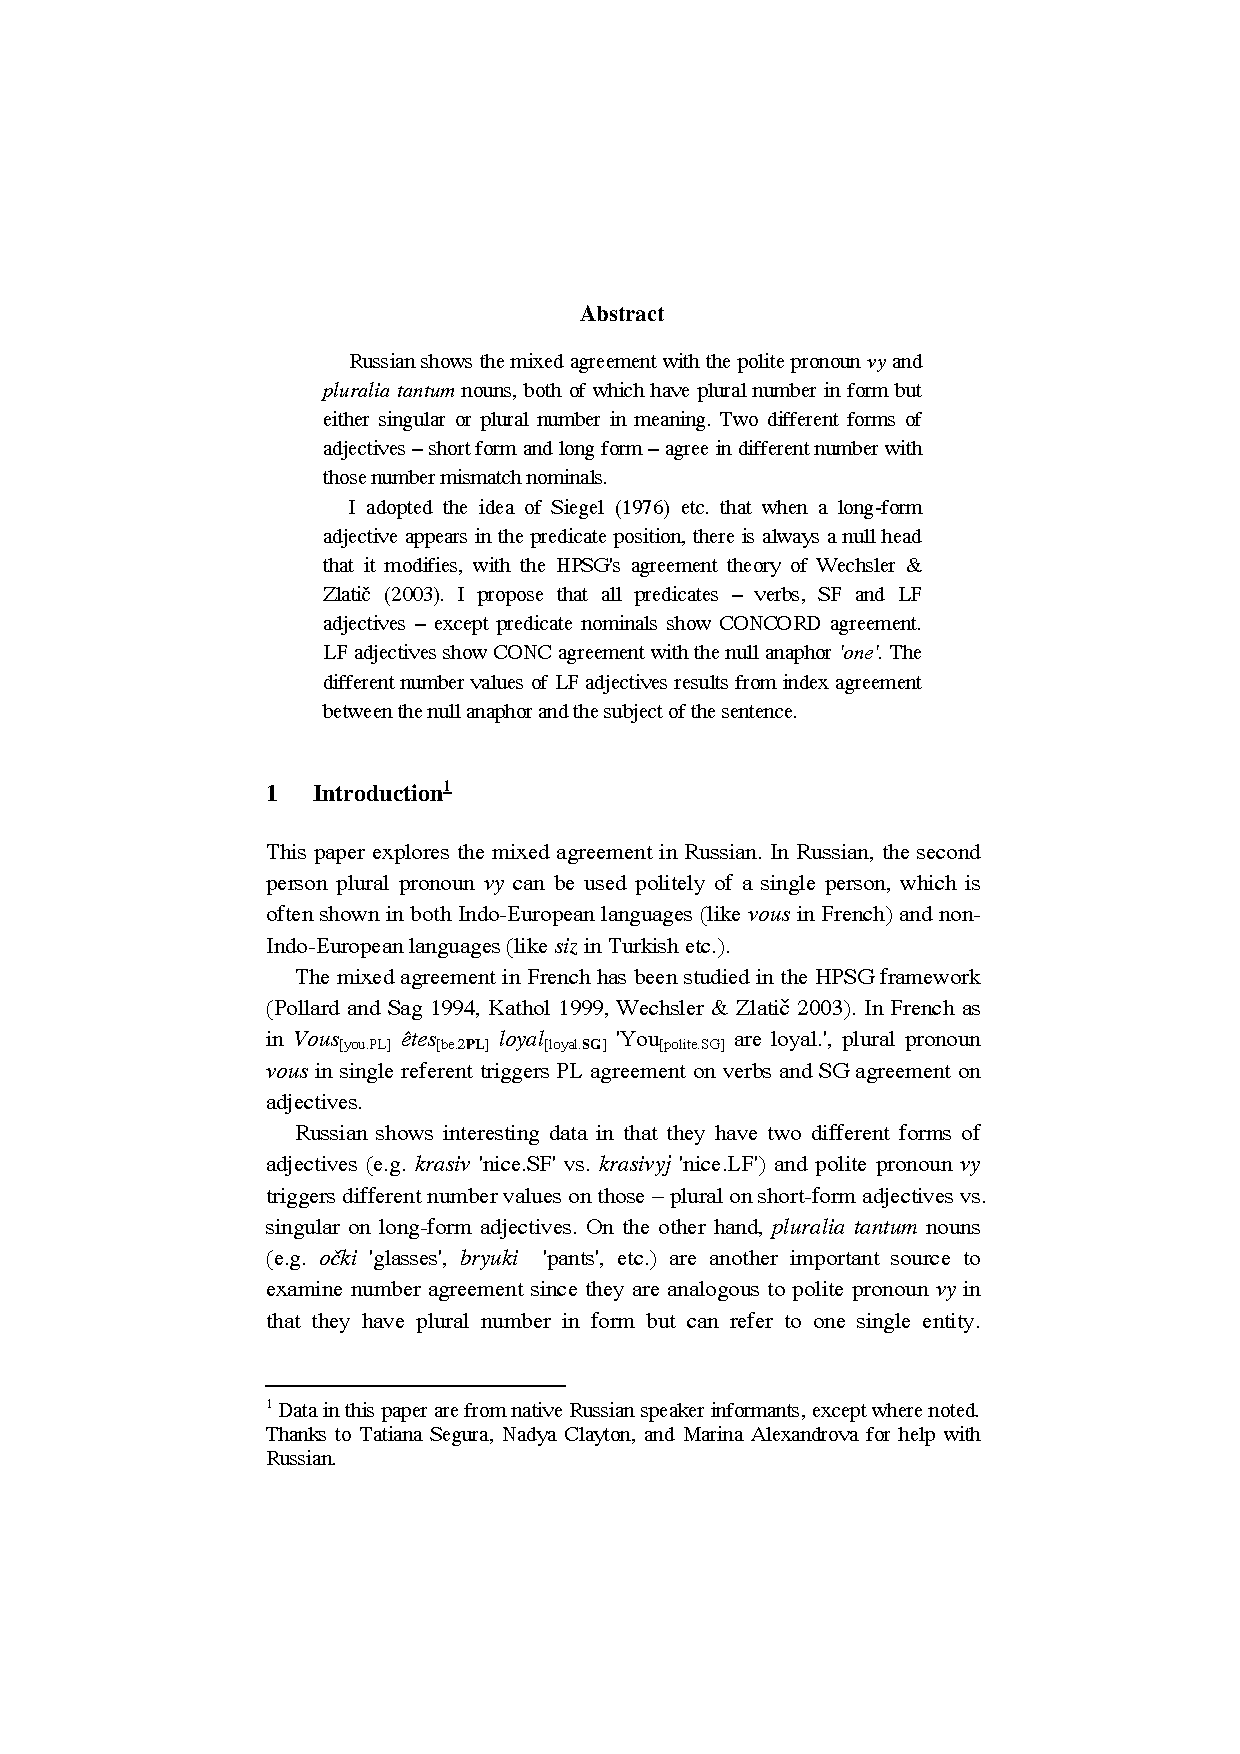
\includepdf[pages=-,pagecommand=\thispagestyle{plain}]{Includes/hahm-hyun-jong.pdf}
        \setcounter{page}{421}
        \phantomsection
        \addcontentsline{toc}{section}{Frank Richter, Jan-Philipp Soehn: \emph{Braucht niemanden zu scheren}: A Survey of NPI Licensing in German}
\thispagestyle{empty}

\begin{center}
  {\huge\bfseries \emph{Braucht niemanden zu scheren}: A Survey of NPI Licensing in German\par}

  \bigskip

~\\
\begingroup
\setlength{\leftskip}{0pt plus 1fill}
\setlength{\rightskip}{0pt plus 1fill}
\setlength{\parindent}{0pt}
\setlength{\parfillskip}{0pt}
  \formatauthor{Frank Richter}{\begin{tabular}{@{}c@{}}University of Tübingen\end{tabular}}
\formatauthor{Jan-Philipp Soehn}{\begin{tabular}{@{}c@{}}University of Tübingen\end{tabular}}

\par\endgroup

  \vspace*{8ex}

  Proceedings of the 13th International Conference on\par Head-Driven Phrase Structure Grammar

  \bigskip

  Linguistic Modelling Laboratory,\\Institute for Parallel Processing,\\Bulgarian Academy of Sciences,\\Sofia,\\Held in Varna

  \medskip

  Stefan Müller (Editor)

  \medskip

  2006

  \medskip

  CSLI Publications

  \medskip

  pages 421--440

  \medskip

  \url{http://csli-publications.stanford.edu/HPSG/2006}
\end{center}
\vfill

\noindent



\vfill
\noindent
% APA Style
Richter, Frank, \& Soehn, Jan-Philipp. 2006. \emph{Braucht niemanden zu scheren}: A Survey of NPI Licensing in German. In Müller, Stefan (Ed.), \emph{{Proceedings of the 13th International Conference on Head-Driven Phrase Structure Grammar, Varna}}, 421--440. Stanford,
CA: CSLI Publications. \hfill\href{http://creativecommons.org/licenses/by/4.0/}{\includegraphics[height=.75em]{Includes/ccby.eps}}

\newpage
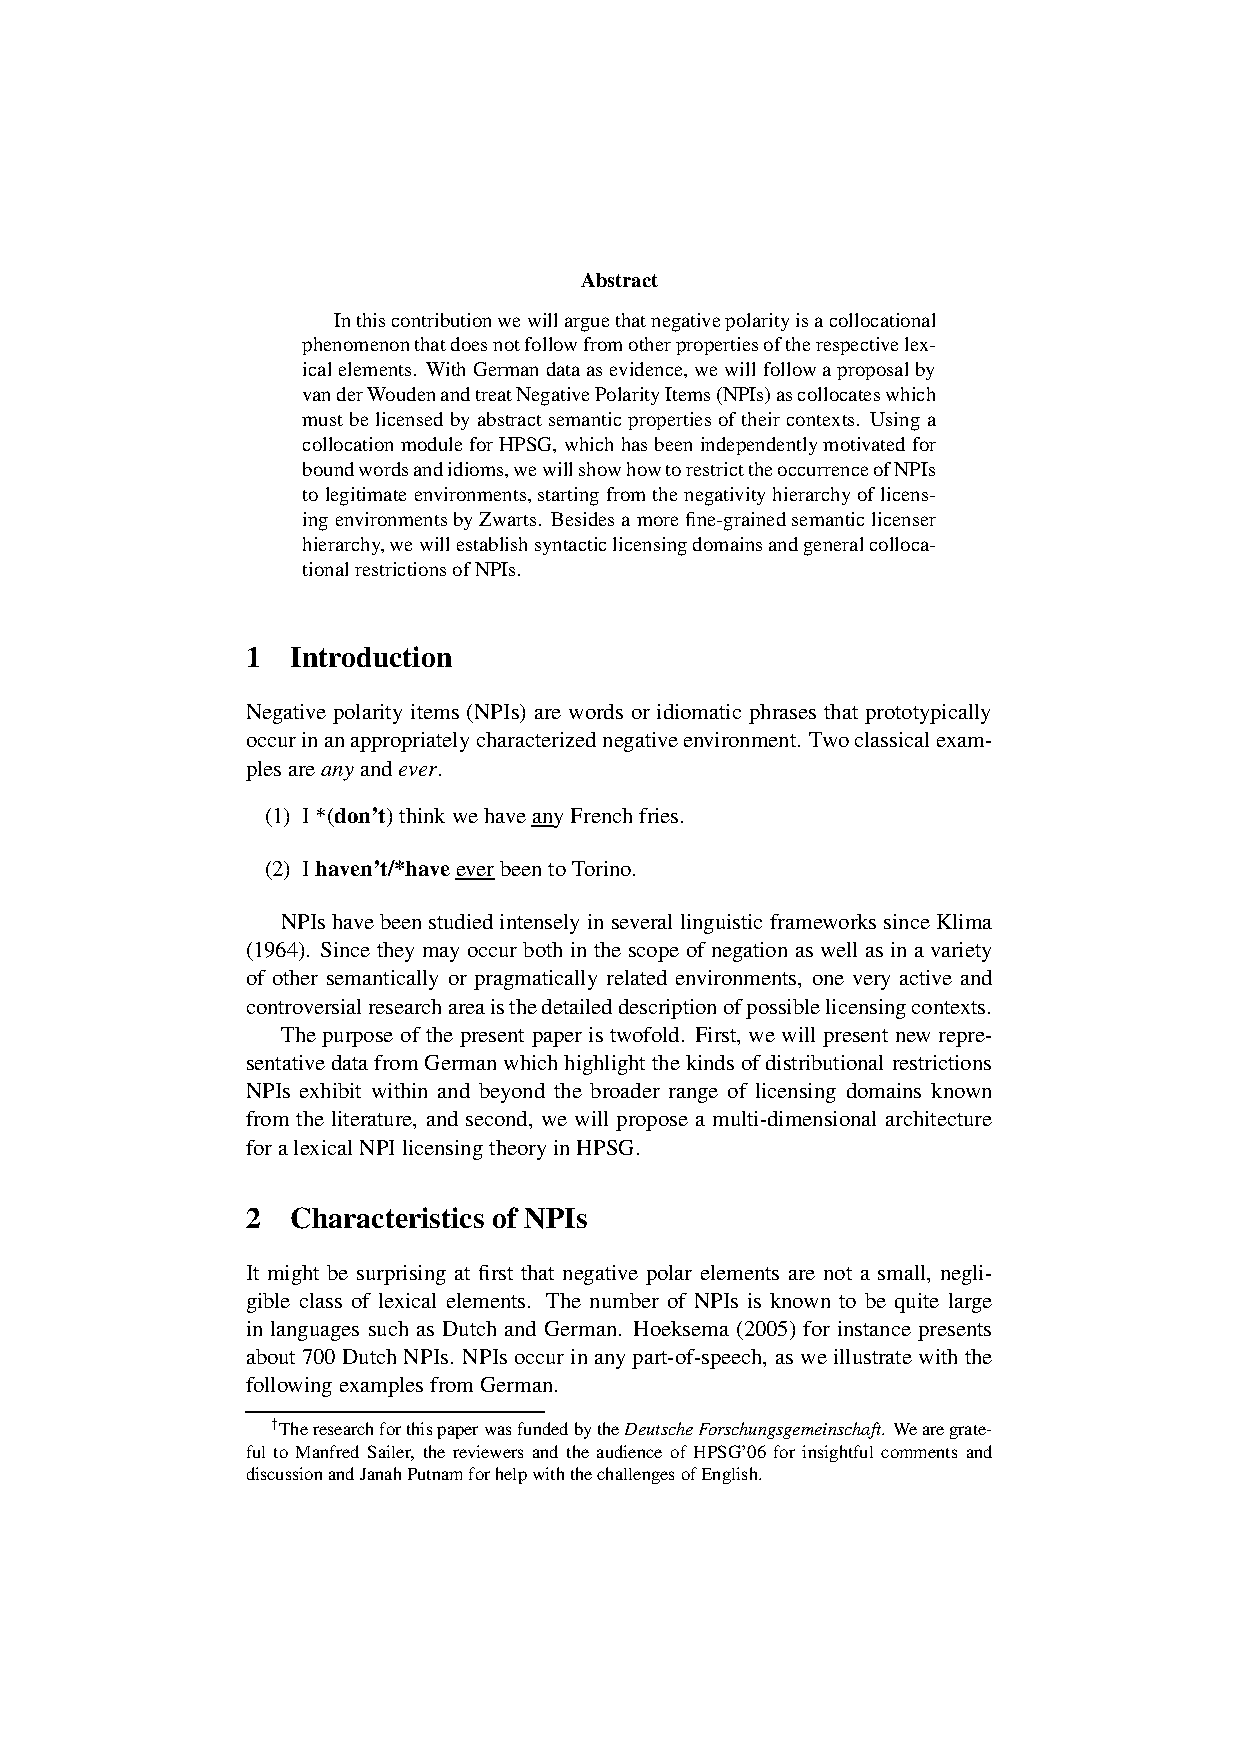
\includepdf[pages=-,pagecommand=\thispagestyle{plain}]{Includes/richter-soehn.pdf}
        \setcounter{page}{441}
        \phantomsection
        \addcontentsline{toc}{section}{Tzvetomira Venkova: Unexpressed Object Alternations of Bulgarian verbs in HPSG}
\thispagestyle{empty}

\begin{center}
  {\huge\bfseries Unexpressed Object Alternations of Bulgarian verbs in HPSG\par}

  \bigskip

~\\
\begingroup
\setlength{\leftskip}{0pt plus 1fill}
\setlength{\rightskip}{0pt plus 1fill}
\setlength{\parindent}{0pt}
\setlength{\parfillskip}{0pt}
  \formatauthor{Tzvetomira Venkova}{\begin{tabular}{@{}c@{}}Sofia University St. Kliment Ohridski\end{tabular}}

\par\endgroup

  \vspace*{8ex}

  Proceedings of the 13th International Conference on\par Head-Driven Phrase Structure Grammar

  \bigskip

  Linguistic Modelling Laboratory,\\Institute for Parallel Processing,\\Bulgarian Academy of Sciences,\\Sofia,\\Held in Varna

  \medskip

  Stefan Müller (Editor)

  \medskip

  2006

  \medskip

  CSLI Publications

  \medskip

  pages 441--455

  \medskip

  \url{http://csli-publications.stanford.edu/HPSG/2006}
\end{center}
\vfill

\noindent



\vfill
\noindent
% APA Style
Venkova, Tzvetomira. 2006. Unexpressed Object Alternations of Bulgarian verbs in HPSG. In Müller, Stefan (Ed.), \emph{{Proceedings of the 13th International Conference on Head-Driven Phrase Structure Grammar, Varna}}, 441--455. Stanford,
CA: CSLI Publications. \hfill\href{http://creativecommons.org/licenses/by/4.0/}{\includegraphics[height=.75em]{Includes/ccby.eps}}

\newpage
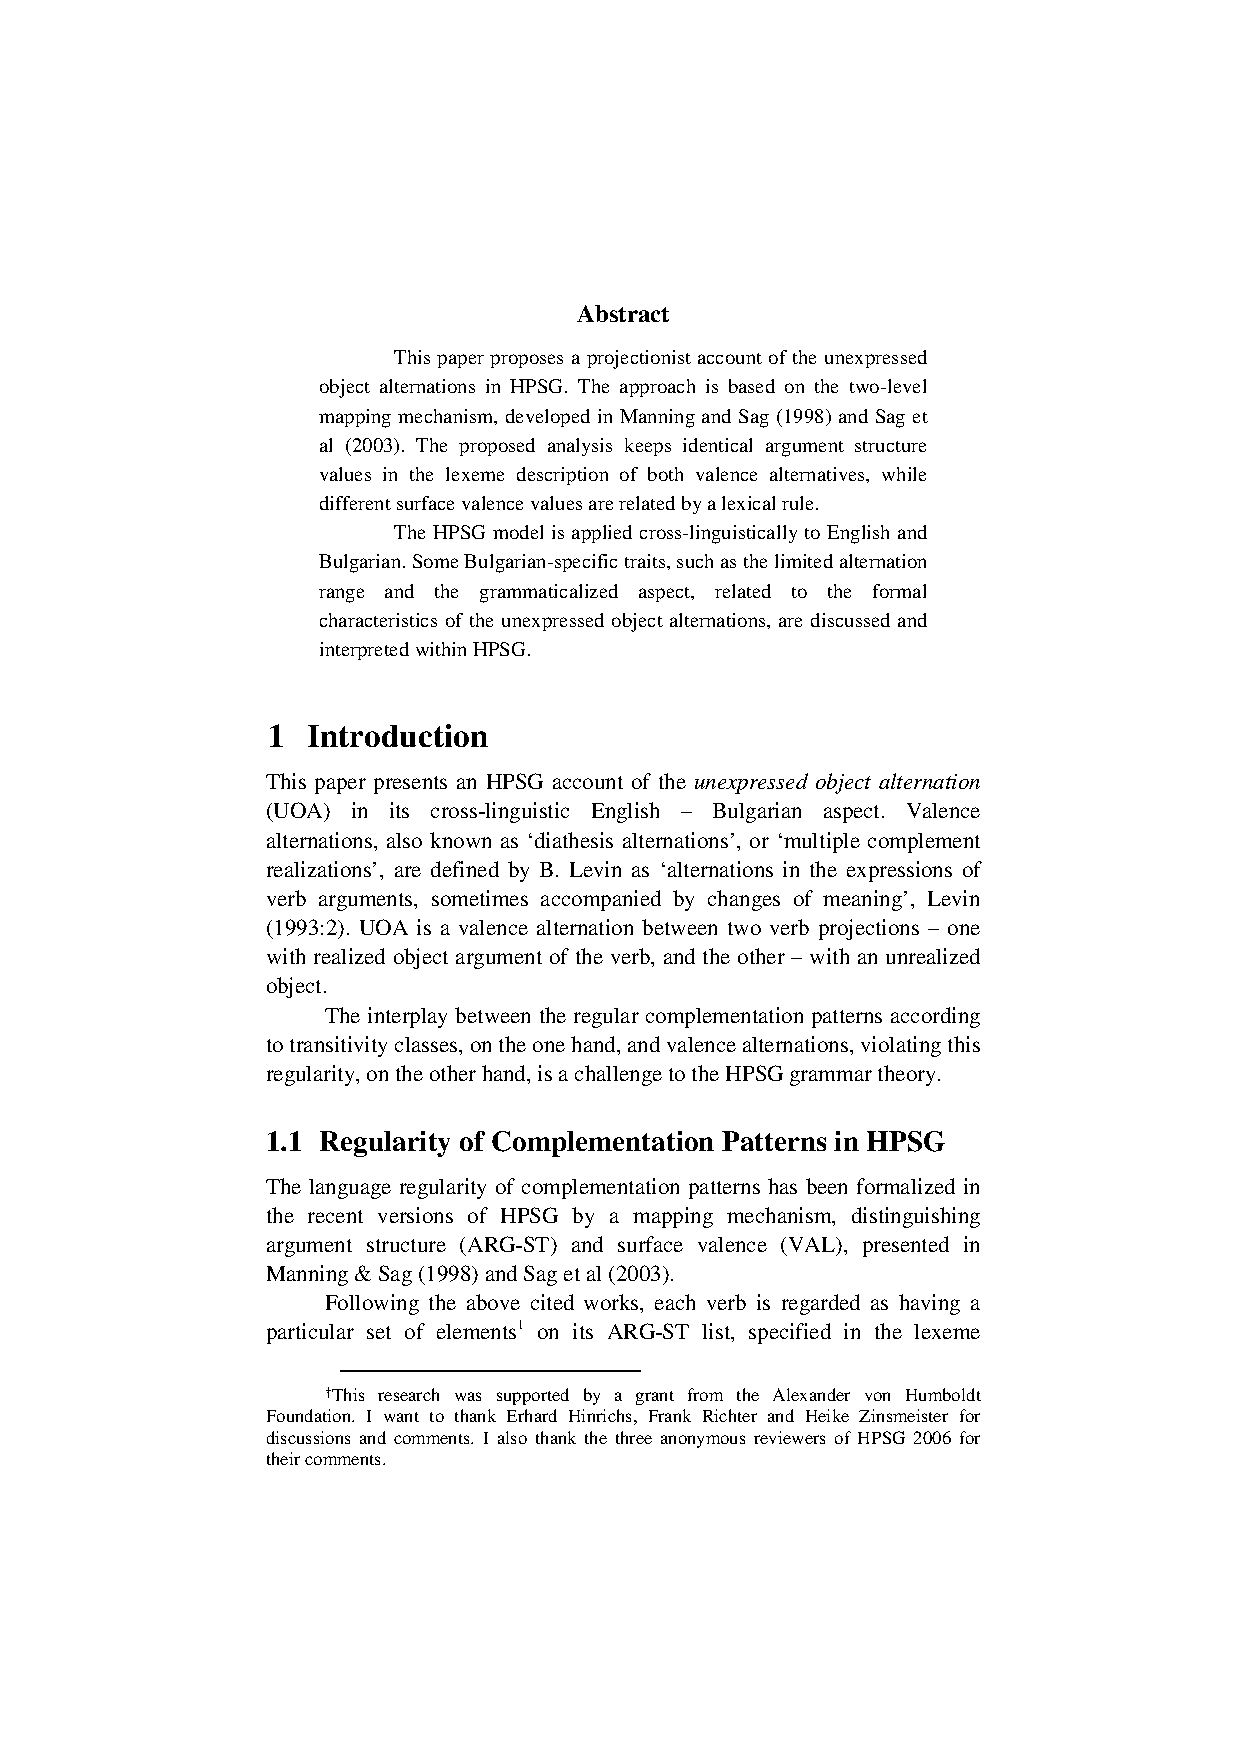
\includepdf[pages=-,pagecommand=\thispagestyle{plain}]{Includes/venkova.pdf}
\end{document}
